\PassOptionsToPackage{dvipsnames}{xcolor}
\documentclass{article}\usepackage[]{graphicx}\usepackage[]{color}
% maxwidth is the original width if it is less than linewidth
% otherwise use linewidth (to make sure the graphics do not exceed the margin)
\makeatletter
\def\maxwidth{ %
  \ifdim\Gin@nat@width>\linewidth
    \linewidth
  \else
    \Gin@nat@width
  \fi
}
\makeatother

\definecolor{fgcolor}{rgb}{0.345, 0.345, 0.345}
\newcommand{\hlnum}[1]{\textcolor[rgb]{0.686,0.059,0.569}{#1}}%
\newcommand{\hlstr}[1]{\textcolor[rgb]{0.192,0.494,0.8}{#1}}%
\newcommand{\hlcom}[1]{\textcolor[rgb]{0.678,0.584,0.686}{\textit{#1}}}%
\newcommand{\hlopt}[1]{\textcolor[rgb]{0,0,0}{#1}}%
\newcommand{\hlstd}[1]{\textcolor[rgb]{0.345,0.345,0.345}{#1}}%
\newcommand{\hlkwa}[1]{\textcolor[rgb]{0.161,0.373,0.58}{\textbf{#1}}}%
\newcommand{\hlkwb}[1]{\textcolor[rgb]{0.69,0.353,0.396}{#1}}%
\newcommand{\hlkwc}[1]{\textcolor[rgb]{0.333,0.667,0.333}{#1}}%
\newcommand{\hlkwd}[1]{\textcolor[rgb]{0.737,0.353,0.396}{\textbf{#1}}}%
\let\hlipl\hlkwb

\usepackage{framed}
\makeatletter
\newenvironment{kframe}{%
 \def\at@end@of@kframe{}%
 \ifinner\ifhmode%
  \def\at@end@of@kframe{\end{minipage}}%
  \begin{minipage}{\columnwidth}%
 \fi\fi%
 \def\FrameCommand##1{\hskip\@totalleftmargin \hskip-\fboxsep
 \colorbox{shadecolor}{##1}\hskip-\fboxsep
     % There is no \\@totalrightmargin, so:
     \hskip-\linewidth \hskip-\@totalleftmargin \hskip\columnwidth}%
 \MakeFramed {\advance\hsize-\width
   \@totalleftmargin\z@ \linewidth\hsize
   \@setminipage}}%
 {\par\unskip\endMakeFramed%
 \at@end@of@kframe}
\makeatother

\definecolor{shadecolor}{rgb}{.97, .97, .97}
\definecolor{messagecolor}{rgb}{0, 0, 0}
\definecolor{warningcolor}{rgb}{1, 0, 1}
\definecolor{errorcolor}{rgb}{1, 0, 0}
\newenvironment{knitrout}{}{} % an empty environment to be redefined in TeX

\usepackage{alltt}
\usepackage{graphicx}
\usepackage{tikz}
\usetikzlibrary{decorations.pathreplacing}
\usepackage{booktabs}
\usepackage{float}
\usepackage[style=apa, natbib]{biblatex}
  \addbibresource{/Users/mk/Dropbox/Papers/mk.bib}

%\usepackage[dvipsnames]{xcolor}
\usepackage{mdframed}
\mdfdefinestyle{style2}{backgroundcolor=gray!10}

\usepackage{xspace}
\newcommand{\code}[1]{\textup{\texttt{\textcolor{violet}{#1}}}}

\usepackage{hyperref}
\usepackage[capitalize, noabbrev]{cleveref}
\usepackage{minitoc}

\newcommand\myshade{85}
\colorlet{mylinkcolor}{violet}
\colorlet{mycitecolor}{YellowOrange}
\colorlet{myurlcolor}{Aquamarine}

\hypersetup{
  linkcolor  = mylinkcolor!\myshade!black,
  citecolor  = mycitecolor!\myshade!black,
  urlcolor   = myurlcolor!\myshade!black,
  colorlinks = true,
}

\title{A model data analysis: Ego depletion}
\author{MK}
\IfFileExists{upquote.sty}{\usepackage{upquote}}{}
\begin{document}

\maketitle

\dosecttoc
\tableofcontents 

\pagebreak





\section{Ego depletion}

Ego depletion is widely-debated topic in the psychological literature. It refers to the claim that people have less self-control in one domain after having to control themselves in another domain of their lives. Thus, one might expect that a person who performs a task that requires self-control (such as the suppression of thoughts, emotions, behavioral impulses, and habits) may not be able to exercise as much self-control in a subsequent task as a person who had not been required to engage in self-control. For example, people who had resisted tempting food, subsequently ate a larger amount of palatable (but unhealthy) food. Because it has been difficult to replicate studies of ego depletion, a group of psychologists in 23 labs independently conducted experiments using an agreed-upon standardized experimental method.

\begin{mdframed}[frametitle = Method of the multilab replication of the ego-depletion effect, style = style2]\label{box:anExperiment}
\sloppy
\mdfsubtitle[subtitlefont = \bfseries\itshape, subtitlebackgroundcolor = gray!10, subtitleaboveskip = 0, subtitlebelowskip = 0]{Data Collection}
Participants were randomly allocated to experimental (ego-depletion) or control (no depletion) groups.

\mdfsubtitle[subtitlefont = \bfseries\itshape, subtitlebackgroundcolor = gray!10, subtitleaboveskip = 0, subtitlebelowskip = 0]{Procedure}
They were told that the experiment was a study of speeded recognition of words and numbers. It consisted of two tasks: the \emph{``\code{e}'' task}, and the \emph{MSIT}, both of which we will describe in a moment. Participants first practiced 20 trials from each tasks. Then they did the ``\code{e}'' task, after which they rated how effortful, fatiguing, difficult, and frustrating it had been. They then did the second task.

\mdfsubtitle[subtitlefont = \bfseries\itshape, subtitlebackgroundcolor = gray!10, subtitleaboveskip = 0, subtitlebelowskip = 0]{Materials}
\emph{The ``\code{e}'' task.} There were two conditions: \emph{depletion} and \emph{no depletion}, in which participants responded to each word as it appeared on the screen. In the depletion condition, they pressed a button when the word contained the letter ``\code{e},'' and refrained from pressing if the ``\code{e}'' was next to or one letter away from a vowel (an example might be the word \code{done}). In the no-depletion version they pressed a button whenever the word contained ``\code{e}'' (for example, \code{done}). The main session consisted of 150 trials and lasted 7.5 minutes.

\emph{Multi-source interference task (MSIT).} The MSIT requires response inhibition. The stimuli were sets of three digits (the numerals \code{1}, \code{2}, \code{3}, or \code{0}). Participants placed their right index, middle, and ring fingers on three keys on the keyboard. On each trial, one of the digits (the \emph{target}; \code{1}, \code{2}, or \code{3}) differed from the two identical \emph{distractors}. They pressed the key corresponding to the target digit. On \emph{congruent} trials, the target matched its position on the keyboard, the distractors were \code{0}s, and the size of the target differed from the distractors (for example: \code{0{\Large 2}0}). On \emph{incongruent} trials, the target did not match its position, the distractors were potential targets, and the different-size digit was not always the target (for example: \code{2{\Large 3}3}). The session consisted of 200 trials (100 congruent and 100 incongruent), which took about 10 minutes.
\end{mdframed}

The data herein were collected by the lab of Mark J. Brandt, Tilburg University, the Netherlands (OSF: \url{https://osf.io/x3y9b/}).

\pagebreak

\section{Import and tidy}

\secttoc

\subsection{\code{e} task}

\subsubsection{Read in}

\begin{knitrout}\footnotesize
\definecolor{shadecolor}{rgb}{0.969, 0.969, 0.969}\color{fgcolor}\begin{kframe}
\begin{alltt}
\hlstd{mkable} \hlkwb{<-} \hlkwa{function}\hlstd{(}\hlkwc{data}\hlstd{) \{}
  \hlstd{knitr}\hlopt{::}\hlkwd{kable}\hlstd{(data,} \hlkwc{booktabs} \hlstd{=} \hlnum{TRUE}\hlstd{,} \hlkwc{digits} \hlstd{=} \hlnum{2}\hlstd{)} \hlopt
    \hlkwd{kable_styling}\hlstd{(}\hlkwc{position} \hlstd{=} \hlstr{"center"}\hlstd{)}
\hlstd{\}}
\hlstd{mkables} \hlkwb{<-} \hlkwa{function}\hlstd{(}\hlkwc{data}\hlstd{) \{}
  \hlstd{knitr}\hlopt{::}\hlkwd{kable}\hlstd{(data,} \hlkwc{booktabs} \hlstd{=} \hlnum{TRUE}\hlstd{,} \hlkwc{digits} \hlstd{=} \hlnum{2}\hlstd{)} \hlopt
    \hlkwd{kable_styling}\hlstd{(}\hlkwc{position} \hlstd{=} \hlstr{"center"}\hlstd{,} \hlkwc{latex_options} \hlstd{=} \hlstr{"scale_down"}\hlstd{)}
\hlstd{\}}
\end{alltt}
\end{kframe}
\end{knitrout}

\begin{knitrout}\footnotesize
\definecolor{shadecolor}{rgb}{0.969, 0.969, 0.969}\color{fgcolor}\begin{kframe}
\begin{alltt}
\hlstd{letE} \hlkwb{<-}
  \hlkwd{read.delim}\hlstd{(}\hlstr{"~/Dropbox/StatsBook/Book5/EgoDepletion/LetterE_EData.txt"}\hlstd{,}
    \hlkwc{fileEncoding} \hlstd{=} \hlstr{"UTF-16"}
  \hlstd{)}
\hlcom{# letE should be in package}
\hlkwd{glimpse}\hlstd{(letE)}
\end{alltt}
\begin{verbatim}
Observations: 24,750
Variables: 35
$ ExperimentName          <fct> LetterETaskt_150_3_easy_NL, LetterETaskt_15...
$ Subject                 <int> 1, 1, 1, 1, 1, 1, 1, 1, 1, 1, 1, 1, 1, 1, 1...
$ Session                 <int> 1, 1, 1, 1, 1, 1, 1, 1, 1, 1, 1, 1, 1, 1, 1...
$ Clock.Information       <fct> <?xml version=1.0?>\n<Clock xmlns:dt=urn:sc...
$ DataFile.Basename       <fct> LetterETaskt_150_3_easy_NL-1-1, LetterETask...
$ Display.RefreshRate     <dbl> 60.001, 60.001, 60.001, 60.001, 60.001, 60....
$ ExperimentVersion       <fct> 1.0.0.63, 1.0.0.63, 1.0.0.63, 1.0.0.63, 1.0...
$ Group                   <int> 1, 1, 1, 1, 1, 1, 1, 1, 1, 1, 1, 1, 1, 1, 1...
$ RandomSeed              <int> 985805828, 985805828, 985805828, 985805828,...
$ RuntimeVersion          <fct> 2.0.10.353, 2.0.10.353, 2.0.10.353, 2.0.10....
$ RuntimeVersionExpected  <fct> 2.0.10.242, 2.0.10.242, 2.0.10.242, 2.0.10....
$ SessionDate             <fct> 03-30-2015, 03-30-2015, 03-30-2015, 03-30-2...
$ SessionStartDateTimeUtc <fct> 30-3-2015 7:07:29, 30-3-2015 7:07:29, 30-3-...
$ SessionTime             <fct> 09:07:29, 09:07:29, 09:07:29, 09:07:29, 09:...
$ StudioVersion           <fct> 2.0.10.147, 2.0.10.147, 2.0.10.147, 2.0.10....
$ Block                   <int> 1, 2, 3, 4, 5, 6, 7, 8, 9, 10, 11, 12, 13, ...
$ Procedure               <fct> ShowStim, ShowStim, ShowStim, ShowStim, Sho...
$ Running                 <fct> WordList, WordList, WordList, WordList, Wor...
$ target                  <int> 1, 1, 1, 1, NA, 1, 1, NA, 1, 1, 1, 1, 1, 1,...
$ TrialNum                <int> 1, 2, 3, 4, 5, 6, 7, 8, 9, 10, 11, 12, 13, ...
$ TrialType               <int> 3, 3, 2, 3, 1, 3, 2, 1, 3, 3, 3, 2, 2, 3, 1...
$ TrialTypeC              <fct> Lonely, Lonely, Companioned, Lonely, NoE, L...
$ Word                    <fct> scheppen, gebruikt, omstandigheid, zuster, ...
$ Word.ACC                <int> 1, 1, 1, 1, 0, 1, 1, 0, 1, 1, 1, 1, 1, 1, 0...
$ Word.CRESP              <int> 1, 1, 1, 1, NA, 1, 1, NA, 1, 1, 1, 1, 1, 1,...
$ Word.DurationError      <int> -7, -7, -7, -7, -7, -7, -7, -7, -7, -7, -7,...
$ Word.OnsetDelay         <int> 7, 7, 7, 7, 7, 7, 7, 7, 7, 7, 7, 7, 7, 7, 7...
$ Word.OnsetTime          <int> 13449, 16449, 19449, 22449, 25449, 28449, 3...
$ Word.OnsetToOnsetTime   <int> 1500, 1500, 1500, 1500, 1500, 1500, 1500, 1...
$ Word.RESP               <int> 1, 1, 1, 1, NA, 1, 1, NA, 1, 1, 1, 1, 1, 1,...
$ Word.RT                 <int> 625, 425, 729, 537, 0, 457, 417, 0, 336, 38...
$ Word.RTTime             <int> 14074, 16874, 20178, 22986, 0, 28906, 31866...
$ WordList                <int> 1, 2, 3, 4, 5, 6, 7, 8, 9, 10, 11, 12, 13, ...
$ WordList.Cycle          <int> 1, 1, 1, 1, 1, 1, 1, 1, 1, 1, 1, 1, 1, 1, 1...
$ WordList.Sample         <int> 1, 2, 3, 4, 5, 6, 7, 8, 9, 10, 11, 12, 13, ...
\end{verbatim}
\end{kframe}
\end{knitrout}

Note: \code{UTF-16} allows us to read a wide range of characters, such as used in text not coded in Latin-script alphabets, and also Greek, Cyrillic, Coptic, Armenian, Hebrew, Arabic, Syriac (roughly equivalent to Aramaic), Thaana (Maldives), and N'Ko (Manding languages). We need it here, because the data were collected in a Dutch-language setting.

\subsubsection{Tidy}

\begin{knitrout}\footnotesize
\definecolor{shadecolor}{rgb}{0.969, 0.969, 0.969}\color{fgcolor}\begin{kframe}
\begin{alltt}
\hlstd{eTask} \hlkwb{<-} \hlkwd{as_tibble}\hlstd{(letE)} \hlopt
  \hlkwd{replace_na}\hlstd{(}\hlkwd{list}\hlstd{(}\hlkwc{Word.RESP} \hlstd{=} \hlnum{0}\hlstd{,} \hlkwc{Word.CRESP} \hlstd{=} \hlnum{0}\hlstd{))}
\hlstd{eTask} \hlkwb{<-} \hlstd{eTask} \hlopt
  \hlkwd{mutate}\hlstd{(}
    \hlkwc{taskDifficulty} \hlstd{=} \hlkwd{as_factor}\hlstd{(}
      \hlkwd{case_when}\hlstd{(}
        \hlstd{ExperimentName} \hlopt{==} \hlstr{"LetterETaskt_150_3_hard_NL"} \hlopt{~} \hlstr{"Hard"}\hlstd{,}
        \hlstd{ExperimentName} \hlopt{==} \hlstr{"LetterETaskt_150_3_easy_NL"} \hlopt{~} \hlstr{"Easy"}
      \hlstd{)}
    \hlstd{),}
    \hlkwc{goNoGo} \hlstd{=} \hlkwd{as_factor}\hlstd{(}
      \hlkwd{case_when}\hlstd{(}
        \hlstd{taskDifficulty} \hlopt{==} \hlstr{"Easy"} \hlopt{&} \hlstd{TrialType} \hlopt \hlkwd{c}\hlstd{(}\hlnum{2}\hlstd{,} \hlnum{3}\hlstd{)} \hlopt{~} \hlstr{"Go"}\hlstd{,}
        \hlstd{taskDifficulty} \hlopt{==} \hlstr{"Hard"} \hlopt{&} \hlstd{TrialType} \hlopt \hlkwd{c}\hlstd{(}\hlnum{3}\hlstd{)} \hlopt{~} \hlstr{"Go"}\hlstd{,}
        \hlstd{taskDifficulty} \hlopt{==} \hlstr{"Easy"} \hlopt{&} \hlstd{TrialType} \hlopt \hlkwd{c}\hlstd{(}\hlnum{1}\hlstd{)} \hlopt{~} \hlstr{"NoGo"}\hlstd{,}
        \hlstd{taskDifficulty} \hlopt{==} \hlstr{"Hard"} \hlopt{&} \hlstd{TrialType} \hlopt \hlkwd{c}\hlstd{(}\hlnum{1}\hlstd{,} \hlnum{2}\hlstd{)} \hlopt{~} \hlstr{"NoGo"}
      \hlstd{)}
    \hlstd{),}
    \hlkwc{displayType} \hlstd{=} \hlkwd{as_factor}\hlstd{(}
      \hlkwd{case_when}\hlstd{(}
        \hlstd{TrialTypeC} \hlopt{==} \hlstr{"Lonely"} \hlopt{~} \hlstr{"NoFlankers"}\hlstd{,}
        \hlstd{TrialTypeC} \hlopt{==} \hlstr{"Companioned"} \hlopt{~} \hlstr{"Flankers"}\hlstd{,}
        \hlstd{TrialTypeC} \hlopt{==} \hlstr{"Lonely"} \hlopt{~} \hlstr{"NoE"}
      \hlstd{)}
    \hlstd{),}
    \hlkwc{sigDet} \hlstd{=} \hlkwd{as_factor}\hlstd{(}
      \hlkwd{case_when}\hlstd{(}
        \hlstd{Word.RESP} \hlopt{==} \hlnum{1} \hlopt{&} \hlstd{Word.CRESP} \hlopt{==} \hlnum{1} \hlopt{~} \hlstr{"Hit"}\hlstd{,}
        \hlstd{Word.RESP} \hlopt{==} \hlnum{0} \hlopt{&} \hlstd{Word.CRESP} \hlopt{==} \hlnum{1} \hlopt{~} \hlstr{"Miss"}\hlstd{,}
        \hlstd{Word.RESP} \hlopt{==} \hlnum{1} \hlopt{&} \hlstd{Word.CRESP} \hlopt{==} \hlnum{0} \hlopt{~} \hlstr{"FA"}\hlstd{,}
        \hlstd{Word.RESP} \hlopt{==} \hlnum{0} \hlopt{&} \hlstd{Word.CRESP} \hlopt{==} \hlnum{0} \hlopt{~} \hlstr{"CR"}
      \hlstd{)}
    \hlstd{),}
    \hlkwc{signalNoise} \hlstd{=} \hlkwd{as_factor}\hlstd{(}
      \hlkwd{case_when}\hlstd{(}
        \hlstd{Word.CRESP} \hlopt{==} \hlnum{1} \hlopt{~} \hlstr{"Signal"}\hlstd{,}
        \hlstd{Word.CRESP} \hlopt{==} \hlnum{0} \hlopt{~} \hlstr{"Noise"}
      \hlstd{)}
    \hlstd{),}
    \hlkwc{subject} \hlstd{=} \hlkwd{as_factor}\hlstd{(Subject),}
    \hlkwc{reactionTime} \hlstd{= Word.RT,}
    \hlkwc{trialNumber} \hlstd{= TrialNum}
  \hlstd{)} \hlopt
  \hlkwd{select}\hlstd{(}
    \hlkwd{c}\hlstd{(}
      \hlstd{taskDifficulty,}
      \hlstd{subject,}
      \hlstd{goNoGo,}
      \hlstd{displayType,}
      \hlstd{sigDet,}
      \hlstd{signalNoise,}
      \hlstd{reactionTime}
    \hlstd{)}
  \hlstd{)}
\hlkwd{glimpse}\hlstd{(eTask)}
\end{alltt}
\begin{verbatim}
Observations: 24,750
Variables: 7
$ taskDifficulty <fct> Easy, Easy, Easy, Easy, Easy, Easy, Easy, Easy, Easy...
$ subject        <fct> 1, 1, 1, 1, 1, 1, 1, 1, 1, 1, 1, 1, 1, 1, 1, 1, 1, 1...
$ goNoGo         <fct> Go, Go, Go, Go, NoGo, Go, Go, NoGo, Go, Go, Go, Go, ...
$ displayType    <fct> NoFlankers, NoFlankers, Flankers, NoFlankers, NA, No...
$ sigDet         <fct> Hit, Hit, Hit, Hit, CR, Hit, Hit, CR, Hit, Hit, Hit,...
$ signalNoise    <fct> Signal, Signal, Signal, Signal, Noise, Signal, Signa...
$ reactionTime   <int> 625, 425, 729, 537, 0, 457, 417, 0, 336, 384, 344, 5...
\end{verbatim}
\end{kframe}
\end{knitrout}

\subsection{MSIT task}

\subsubsection{Read in}

\begin{knitrout}\footnotesize
\definecolor{shadecolor}{rgb}{0.969, 0.969, 0.969}\color{fgcolor}\begin{kframe}
\begin{alltt}
\hlstd{msit} \hlkwb{<-}
  \hlkwd{read.delim}\hlstd{(}
    \hlkwc{file} \hlstd{=} \hlstr{"~/Dropbox/StatsBook/Book5/EgoDepletion/MSIT200_EData.txt"}\hlstd{,}
    \hlkwc{fileEncoding} \hlstd{=} \hlstr{"UTF-16"}
  \hlstd{)}
\hlkwd{glimpse}\hlstd{(msit)}
\end{alltt}
\begin{verbatim}
Observations: 33,000
Variables: 41
$ ExperimentName          <fct> MAS_MSIT_event_200_3_NL, MAS_MSIT_event_200...
$ Subject                 <int> 1, 1, 1, 1, 1, 1, 1, 1, 1, 1, 1, 1, 1, 1, 1...
$ Session                 <int> 1, 1, 1, 1, 1, 1, 1, 1, 1, 1, 1, 1, 1, 1, 1...
$ Clock.Information       <fct> <?xml version=1.0?>\n<Clock xmlns:dt=urn:sc...
$ DataFile.Basename       <fct> MAS_MSIT_event_200_3_NL-1-1, MAS_MSIT_event...
$ Display.RefreshRate     <dbl> 60.001, 60.001, 60.001, 60.001, 60.001, 60....
$ ExperimentVersion       <fct> 1.0.0.43, 1.0.0.43, 1.0.0.43, 1.0.0.43, 1.0...
$ Group                   <int> 1, 1, 1, 1, 1, 1, 1, 1, 1, 1, 1, 1, 1, 1, 1...
$ RandomSeed              <int> -1687224442, -1687224442, -1687224442, -168...
$ RuntimeVersion          <fct> 2.0.10.353, 2.0.10.353, 2.0.10.353, 2.0.10....
$ RuntimeVersionExpected  <fct> 2.0.10.242, 2.0.10.242, 2.0.10.242, 2.0.10....
$ SessionDate             <fct> 03-30-2015, 03-30-2015, 03-30-2015, 03-30-2...
$ SessionStartDateTimeUtc <fct> 30-3-2015 7:16:57, 30-3-2015 7:16:57, 30-3-...
$ SessionTime             <fct> 09:16:57, 09:16:57, 09:16:57, 09:16:57, 09:...
$ StudioVersion           <fct> 2.0.10.147, 2.0.10.147, 2.0.10.147, 2.0.10....
$ Block                   <int> 1, 2, 3, 4, 5, 6, 7, 8, 9, 10, 11, 12, 13, ...
$ content                 <int> 100, 3, 311, 212, 322, 331, 3, 100, 3, 211,...
$ Digits.ACC              <int> 1, 1, 0, 0, 0, 0, 1, 1, 1, 0, 0, 0, 1, 1, 1...
$ Digits.CRESP            <int> 1, 3, 3, 1, 3, 1, 3, 1, 3, 2, 2, 2, 2, 3, 1...
$ Digits.DurationError    <int> -6, -6, -6, -6, -6, -6, -6, -6, -6, -6, -6,...
$ Digits.OnsetDelay       <int> 6, 6, 6, 6, 6, 6, 6, 6, 6, 6, 6, 6, 6, 6, 6...
$ Digits.OnsetTime        <int> 24021, 27021, 30021, 33021, 36021, 39021, 4...
$ Digits.OnsetToOnsetTime <int> 500, 500, 500, 500, 500, 500, 500, 500, 500...
$ Digits.RESP             <int> 1, 3, 1, 2, 1, 3, 3, 1, 3, 1, 3, 1, 2, 3, 1...
$ Digits.RT               <int> 530, 538, 426, 962, 882, 625, 489, 529, 553...
$ Digits.RTTime           <int> 24551, 27559, 30447, 33983, 36903, 39646, 4...
$ Left                    <int> 1, 0, 3, 2, 3, 3, 0, 1, 0, 2, 1, 2, 0, 0, 1...
$ LeftSize                <int> 28, 20, 28, 28, 20, 20, 20, 28, 20, 20, 20,...
$ Middle                  <int> 0, 0, 1, 1, 2, 3, 0, 0, 0, 1, 1, 3, 2, 0, 0...
$ MiddleSize              <int> 20, 20, 20, 20, 20, 20, 20, 20, 20, 20, 20,...
$ Procedure               <fct> ShowStim, ShowStim, ShowStim, ShowStim, Sho...
$ Right                   <int> 0, 3, 1, 2, 2, 1, 3, 0, 3, 1, 2, 3, 0, 3, 0...
$ RightSize               <int> 20, 28, 20, 20, 28, 28, 28, 20, 28, 28, 28,...
$ Running                 <fct> StimList, StimList, StimList, StimList, Sti...
$ StimList                <int> 1, 2, 3, 4, 5, 6, 7, 8, 9, 10, 11, 12, 13, ...
$ StimList.Cycle          <int> 1, 1, 1, 1, 1, 1, 1, 1, 1, 1, 1, 1, 1, 1, 1...
$ StimList.Sample         <int> 1, 2, 3, 4, 5, 6, 7, 8, 9, 10, 11, 12, 13, ...
$ target                  <int> 1, 3, 3, 1, 3, 1, 3, 1, 3, 2, 2, 2, 2, 3, 1...
$ TrialNum                <int> 1, 2, 3, 4, 5, 6, 7, 8, 9, 10, 11, 12, 13, ...
$ TrialType               <int> 1, 1, 2, 2, 2, 2, 1, 1, 1, 2, 2, 2, 1, 1, 1...
$ TrialTypeC              <fct> C, C, I, I, I, I, C, C, C, I, I, I, C, C, C...
\end{verbatim}
\end{kframe}
\end{knitrout}

\subsubsection{Tidy}

\begin{knitrout}\footnotesize
\definecolor{shadecolor}{rgb}{0.969, 0.969, 0.969}\color{fgcolor}\begin{kframe}
\begin{alltt}
\hlstd{mTask} \hlkwb{<-} \hlkwd{as_tibble}\hlstd{(msit)} \hlopt
  \hlkwd{transmute}\hlstd{(}
    \hlkwc{response} \hlstd{= Digits.RESP,}
    \hlkwc{stimulus} \hlstd{= Digits.CRESP,}
    \hlkwc{sigDet} \hlstd{=} \hlkwd{as_factor}\hlstd{(}
      \hlkwd{case_when}\hlstd{(}
        \hlstd{stimulus} \hlopt{==} \hlstd{response} \hlopt{~} \hlstr{"Hit"}\hlstd{,}
        \hlkwd{abs}\hlstd{(stimulus} \hlopt{-} \hlstd{response)} \hlopt{==} \hlnum{1} \hlopt{~} \hlstr{"FA1"}\hlstd{,}
        \hlkwd{abs}\hlstd{(stimulus} \hlopt{-} \hlstd{response)} \hlopt{==} \hlnum{2} \hlopt{~} \hlstr{"FA2"}
      \hlstd{)}
    \hlstd{),}
    \hlkwc{reactionTime} \hlstd{= Digits.RT,}
    \hlkwc{subject} \hlstd{=} \hlkwd{factor}\hlstd{(Subject),}
    \hlkwc{trialType} \hlstd{=} \hlkwd{as_factor}\hlstd{(}
      \hlkwd{case_when}\hlstd{(}
        \hlstd{TrialTypeC} \hlopt{==} \hlstr{"C"} \hlopt{~} \hlstr{"Congruent"}\hlstd{,}
        \hlstd{TrialTypeC} \hlopt{==} \hlstr{"I"} \hlopt{~} \hlstr{"Incongruent"}
      \hlstd{)}
    \hlstd{)}
  \hlstd{)}
\hlkwd{glimpse}\hlstd{(mTask)}
\end{alltt}
\begin{verbatim}
Observations: 33,000
Variables: 6
$ response     <int> 1, 3, 1, 2, 1, 3, 3, 1, 3, 1, 3, 1, 2, 3, 1, 1, 1, 2, ...
$ stimulus     <int> 1, 3, 3, 1, 3, 1, 3, 1, 3, 2, 2, 2, 2, 3, 1, 3, 2, 1, ...
$ sigDet       <fct> Hit, Hit, FA2, FA1, FA2, FA2, Hit, Hit, Hit, FA1, FA1,...
$ reactionTime <int> 530, 538, 426, 962, 882, 625, 489, 529, 553, 721, 425,...
$ subject      <fct> 1, 1, 1, 1, 1, 1, 1, 1, 1, 1, 1, 1, 1, 1, 1, 1, 1, 1, ...
$ trialType    <fct> Congruent, Congruent, Incongruent, Incongruent, Incong...
\end{verbatim}
\end{kframe}
\end{knitrout}

\subsection{Subject info and ratings}

\subsubsection{Read in}

\begin{knitrout}\footnotesize
\definecolor{shadecolor}{rgb}{0.969, 0.969, 0.969}\color{fgcolor}\begin{kframe}
\begin{alltt}
\hlstd{subs} \hlkwb{<-} \hlkwd{read_csv}\hlstd{(}\hlkwc{file} \hlstd{=} \hlstr{"~/Dropbox/StatsBook/Book5/EgoDepletion/SubjectStatus.csv"}\hlstd{)}
\hlkwd{glimpse}\hlstd{(subs)}
\end{alltt}
\begin{verbatim}
Observations: 165
Variables: 11
$ SubjectID  <dbl> 1, 2, 3, 5, 6, 8, 9, 10, 11, 14, 16, 17, 21, 22, 23, 25,...
$ Task       <chr> "E", "E", "E", "E", "E", "E", "E", "E", "E", "E", "E", "...
$ condition  <dbl> 1, 1, 1, 1, 1, 1, 1, 1, 1, 1, 1, 1, 1, 1, 1, 1, 1, 1, 1,...
$ gender     <dbl> 2, 1, 2, 2, 2, 2, 1, 2, 2, 2, 2, 2, 2, 2, 1, 2, 2, 2, 2,...
$ age        <dbl> 19, 19, 19, 19, 18, 22, 18, 19, 23, 19, 19, 18, 18, 19, ...
$ lang       <dbl> 1, 1, 1, 2, 1, 1, 1, 1, 1, 1, 1, 1, 1, 1, 2, 1, 1, 1, 1,...
$ langother  <chr> NA, NA, NA, "Duits", NA, NA, NA, NA, NA, NA, NA, NA, NA,...
$ effort     <dbl> 2, 5, 5, 2, 3, 2, 2, 4, 2, 2, 3, 2, 6, 3, 3, 3, 3, 5, 2,...
$ difficult  <dbl> 1, 3, 1, 3, 2, 2, 3, 3, 4, 2, 1, 3, 2, 3, 3, 1, 1, 2, 2,...
$ tired      <dbl> 6, 4, 2, 5, 3, 3, 5, 2, 2, 6, 4, 4, 6, 5, 2, 1, 4, 4, 4,...
$ frustrated <dbl> 1, 2, 1, 1, 1, 2, 1, 1, 3, 4, 2, 2, 4, 2, 2, 1, 1, 1, 4,...
\end{verbatim}
\end{kframe}
\end{knitrout}

\subsubsection{Tidy}

\begin{knitrout}\footnotesize
\definecolor{shadecolor}{rgb}{0.969, 0.969, 0.969}\color{fgcolor}\begin{kframe}
\begin{alltt}
\hlstd{subjectInfo} \hlkwb{<-} \hlstd{subs} \hlopt
  \hlkwd{select}\hlstd{(}\hlopt{-}\hlkwd{c}\hlstd{(langother, condition))} \hlopt
  \hlkwd{rename}\hlstd{(}
    \hlkwc{subject} \hlstd{= SubjectID,}
    \hlkwc{effortRating} \hlstd{= effort,}
    \hlkwc{difficultyRating} \hlstd{= difficult,}
    \hlkwc{fatigueRating} \hlstd{= tired,}
    \hlkwc{firstLanguage} \hlstd{= lang,}
    \hlkwc{frustrationRating} \hlstd{= frustrated}
  \hlstd{)} \hlopt
  \hlkwd{mutate}\hlstd{(}
    \hlkwc{subject} \hlstd{=} \hlkwd{factor}\hlstd{(subject),}
    \hlkwc{taskDifficulty} \hlstd{=} \hlkwd{factor}\hlstd{(}
      \hlkwd{case_when}\hlstd{(}
        \hlstd{Task} \hlopt{==} \hlstr{"E"} \hlopt{~} \hlstr{"Easy"}\hlstd{,}
        \hlstd{Task} \hlopt{==} \hlstr{"H"} \hlopt{~} \hlstr{"Hard"}
      \hlstd{)}
    \hlstd{),}
    \hlkwc{gender} \hlstd{=} \hlkwd{factor}\hlstd{(}
      \hlkwd{case_when}\hlstd{(}
        \hlstd{gender} \hlopt{==} \hlnum{1} \hlopt{~} \hlstr{"Male"}\hlstd{,}
        \hlstd{gender} \hlopt{==} \hlnum{2} \hlopt{~} \hlstr{"Female"}
      \hlstd{)}
    \hlstd{),}
  \hlstd{)} \hlopt
  \hlkwd{select}\hlstd{(}
    \hlkwd{c}\hlstd{(}
      \hlstd{taskDifficulty,}
      \hlstd{gender,}
      \hlstd{subject,}
      \hlstd{effortRating,}
      \hlstd{difficultyRating,}
      \hlstd{frustrationRating,}
      \hlstd{fatigueRating}
    \hlstd{)}
  \hlstd{)}
\hlkwd{glimpse}\hlstd{(subjectInfo)}
\end{alltt}
\begin{verbatim}
Observations: 165
Variables: 7
$ taskDifficulty    <fct> Easy, Easy, Easy, Easy, Easy, Easy, Easy, Easy, E...
$ gender            <fct> Female, Male, Female, Female, Female, Female, Mal...
$ subject           <fct> 1, 2, 3, 5, 6, 8, 9, 10, 11, 14, 16, 17, 21, 22, ...
$ effortRating      <dbl> 2, 5, 5, 2, 3, 2, 2, 4, 2, 2, 3, 2, 6, 3, 3, 3, 3...
$ difficultyRating  <dbl> 1, 3, 1, 3, 2, 2, 3, 3, 4, 2, 1, 3, 2, 3, 3, 1, 1...
$ frustrationRating <dbl> 1, 2, 1, 1, 1, 2, 1, 1, 3, 4, 2, 2, 4, 2, 2, 1, 1...
$ fatigueRating     <dbl> 6, 4, 2, 5, 3, 3, 5, 2, 2, 6, 4, 4, 6, 5, 2, 1, 4...
\end{verbatim}
\end{kframe}
\end{knitrout}

\pagebreak

\section{Preliminary description}

\secttoc

\subsection{\code{eTask} data}

\subsubsection{Disregarding subjects}

\paragraph{RT}

\subparagraph{Transform RT?}

Now we would like to get a sense of the mean RTs in these conditions. This cannot be done reasonably unless we assume that these are distributed symmetrically (and preferably normally). But the distribution of RTs is meaningful \emph{only relative to a model.} So we model these data with a linear model. (By doing so, we are --- incorrectly --- treating the data as if they came from one subject.)

\begin{knitrout}\footnotesize
\definecolor{shadecolor}{rgb}{0.969, 0.969, 0.969}\color{fgcolor}\begin{kframe}
\begin{alltt}
\hlstd{eTaskH.FA} \hlkwb{<-} \hlstd{eTask} \hlopt
  \hlkwd{filter}\hlstd{(sigDet} \hlopt{!=} \hlstr{"CR"}\hlstd{)}
\hlstd{lmETaskH.FA} \hlkwb{<-} \hlkwd{lm}\hlstd{(reactionTime} \hlopt{~} \hlstd{taskDifficulty} \hlopt{*} \hlstd{sigDet,} \hlkwc{data} \hlstd{= eTaskH.FA)}
\end{alltt}
\end{kframe}
\end{knitrout}

\noindent Rather than examining the distribution of the residuals from \code{lmETaskHit}, we look for the value of $\lambda$ (the power of the transformation) that will maximize the MLE of the model.

\begin{knitrout}\footnotesize
\definecolor{shadecolor}{rgb}{0.969, 0.969, 0.969}\color{fgcolor}\begin{kframe}
\begin{alltt}
\hlkwd{library}\hlstd{(car)}
\hlkwd{summary}\hlstd{(}\hlkwd{powerTransform}\hlstd{(lmETaskH.FA))}
\end{alltt}
\begin{verbatim}
bcPower Transformation to Normality 
   Est Power Rounded Pwr Wald Lwr Bnd Wald Upr Bnd
Y1   -0.0595       -0.06      -0.0797      -0.0393

Likelihood ratio test that transformation parameter is equal to 0
 (log transformation)
                           LRT df       pval
LR test, lambda = (0) 31.94887  1 1.5828e-08

Likelihood ratio test that no transformation is needed
                          LRT df       pval
LR test, lambda = (1) 7376.75  1 < 2.22e-16
\end{verbatim}
\end{kframe}
\end{knitrout}

\noindent So, should we transform \code{reactionTime}? Yes. Since $\lambda = -0.06 \approx 0$, and in the ladder of powers $\lambda = 0$ means $y \rightarrow \log{y}$. We can also show this graphically (\Cref{fig:eTaskBoxCox}):

\begin{knitrout}\footnotesize
\definecolor{shadecolor}{rgb}{0.969, 0.969, 0.969}\color{fgcolor}\begin{kframe}
\begin{alltt}
\hlkwd{library}\hlstd{(lindia)}
\hlkwd{gg_boxcox}\hlstd{(lmETaskH.FA)}
\end{alltt}
\end{kframe}
\end{knitrout}

\begin{figure}
\begin{knitrout}\footnotesize
\definecolor{shadecolor}{rgb}{0.969, 0.969, 0.969}\color{fgcolor}

{\centering 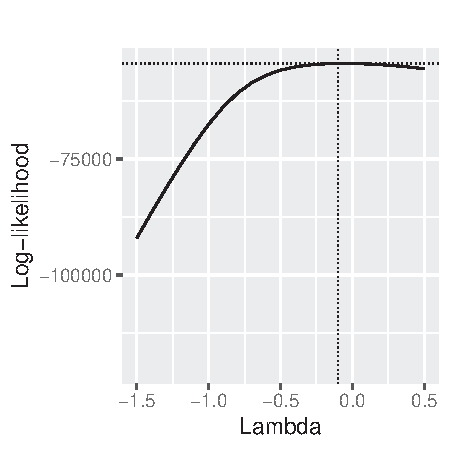
\includegraphics[width=.5\linewidth]{figure/graphics-lm_eTaskHit_boxcox_show-1} 

}



\end{knitrout}
\caption{Plot profile log-likelihoods for the parameter of the Box-Cox power family for \code{lmETaskHit}.}\label{fig:eTaskBoxCox}
\end{figure}

So we transform \code{reactionTime}, and rerun the \code{lm()}:

\begin{knitrout}\footnotesize
\definecolor{shadecolor}{rgb}{0.969, 0.969, 0.969}\color{fgcolor}\begin{kframe}
\begin{alltt}
\hlstd{eTaskH.FA} \hlkwb{<-} \hlstd{eTaskH.FA} \hlopt
  \hlkwd{mutate}\hlstd{(}\hlkwc{reactionTimeLog} \hlstd{=} \hlkwd{log}\hlstd{(reactionTime))}
\hlstd{lmeTaskH.FA.Log} \hlkwb{<-} \hlkwd{update}\hlstd{(}\hlkwc{object} \hlstd{= lmETaskH.FA,} \hlkwc{formula.} \hlstd{= reactionTimeLog} \hlopt{~} \hlstd{.)}
\end{alltt}
\end{kframe}
\end{knitrout}

\noindent (Note that we use \code{update()}.)

\begin{knitrout}\footnotesize
\definecolor{shadecolor}{rgb}{0.969, 0.969, 0.969}\color{fgcolor}\begin{kframe}
\begin{alltt}
\hlkwd{AIC}\hlstd{(lmETaskH.FA, lmeTaskH.FA.Log)} \hlopt
  \hlkwd{as_tibble}\hlstd{()} \hlopt
  \hlkwd{kable}\hlstd{(}\hlkwc{digits} \hlstd{=} \hlnum{0}\hlstd{,} \hlkwc{booktabs} \hlstd{=} \hlnum{TRUE}\hlstd{)} \hlopt
  \hlkwd{kable_styling}\hlstd{(}\hlkwc{position} \hlstd{=} \hlstr{"center"}\hlstd{)}
\end{alltt}
\end{kframe}\begin{table}[H]
\centering
\begin{tabular}{rr}
\toprule
df & AIC\\
\midrule
5 & 210791\\
5 & 6901\\
\bottomrule
\end{tabular}
\end{table}


\end{knitrout}

\noindent We made a point \emph{not} to look at the linear models before determining the difference in AIC, and finding that \code{lmeTaskHitLog} is overwhelmingly better  than \code{lmETaskHit}. We do not have to do this again when we run LME models on these data. (Nevertheless, it's always prudent to double-check by using \code{powerTransform()} on our final model, and confirming that $\lambda \approx 1$, which means that the fit of the model cannot be improved by transforming the response variable.)

Summarize Detection \& RT

\begin{knitrout}\footnotesize
\definecolor{shadecolor}{rgb}{0.969, 0.969, 0.969}\color{fgcolor}\begin{kframe}
\begin{alltt}
\hlstd{eTaskSum} \hlkwb{<-} \hlstd{eTask} \hlopt
  \hlkwd{group_by}\hlstd{(taskDifficulty, signalNoise, sigDet)} \hlopt
  \hlkwd{mutate}\hlstd{(}\hlkwc{reactionTimeLog} \hlstd{=} \hlkwd{log}\hlstd{(reactionTime))} \hlopt
  \hlkwd{summarize}\hlstd{(}\hlkwc{meanRTlog} \hlstd{=} \hlkwd{mean}\hlstd{(reactionTimeLog),} \hlkwc{n} \hlstd{=} \hlkwd{n}\hlstd{())} \hlopt
  \hlkwd{mutate}\hlstd{(}\hlkwc{prop} \hlstd{= n} \hlopt{/} \hlkwd{sum}\hlstd{(n),} \hlkwc{geomMean.eTask.RT} \hlstd{=} \hlkwd{exp}\hlstd{(meanRTlog))} \hlopt
  \hlkwd{filter}\hlstd{(sigDet} \hlopt{!=} \hlstr{"CR"}\hlstd{)} \hlopt
  \hlkwd{select}\hlstd{(}\hlopt{-}\hlkwd{c}\hlstd{(n, meanRTlog))} \hlopt
  \hlkwd{select}\hlstd{(taskDifficulty, sigDet, prop, geomMean.eTask.RT)}
\hlstd{eTaskSum} \hlopt
  \hlkwd{kable}\hlstd{(}\hlkwc{digits} \hlstd{=} \hlkwd{c}\hlstd{(}\hlnum{0}\hlstd{,} \hlnum{0}\hlstd{,} \hlnum{0}\hlstd{,} \hlnum{3}\hlstd{,} \hlnum{0}\hlstd{),} \hlkwc{booktabs} \hlstd{=} \hlnum{TRUE}\hlstd{)} \hlopt
  \hlkwd{kable_styling}\hlstd{(}\hlkwc{position} \hlstd{=} \hlstr{"center"}\hlstd{)}
\end{alltt}
\end{kframe}\begin{table}[H]
\centering
\begin{tabular}{lllrr}
\toprule
signalNoise & taskDifficulty & sigDet & prop & geomMean.eTask.RT\\
\midrule
Signal & Easy & Hit & 1.000 & 542\\
Noise & Easy & FA & 0.064 & 450\\
Signal & Hard & Hit & 1.000 & 1080\\
Noise & Hard & FA & 0.138 & 1072\\
\bottomrule
\end{tabular}
\end{table}


\end{knitrout}

\noindent Clearly none of the subjects made errors when they responded to a word that contained \code{e}, but made more than twice as many inhibition errors in the \code{Hard} condition (13.8\%) than in the \code{Easy} condition (6.4\%).

Now we do this by subject:

\begin{knitrout}\footnotesize
\definecolor{shadecolor}{rgb}{0.969, 0.969, 0.969}\color{fgcolor}\begin{kframe}
\begin{alltt}
\hlstd{eTaskBySub} \hlkwb{<-} \hlstd{eTask} \hlopt
  \hlkwd{group_by}\hlstd{(taskDifficulty, subject, signalNoise, sigDet)} \hlopt
  \hlkwd{mutate}\hlstd{(}\hlkwc{reactionTimeLog} \hlstd{=} \hlkwd{log}\hlstd{(reactionTime))} \hlopt
  \hlkwd{summarize}\hlstd{(}\hlkwc{meanRTlog} \hlstd{=} \hlkwd{mean}\hlstd{(reactionTimeLog),} \hlkwc{n} \hlstd{=} \hlkwd{n}\hlstd{())} \hlopt
  \hlkwd{mutate}\hlstd{(}\hlkwc{prop} \hlstd{= n} \hlopt{/} \hlkwd{sum}\hlstd{(n),} \hlkwc{geomMean.eTask.RT} \hlstd{=} \hlkwd{exp}\hlstd{(meanRTlog))} \hlopt
  \hlkwd{filter}\hlstd{(sigDet} \hlopt{!=} \hlstr{"CR"}\hlstd{)} \hlopt
  \hlkwd{select}\hlstd{(}\hlopt{-}\hlkwd{c}\hlstd{(n, meanRTlog))} \hlopt
  \hlkwd{select}\hlstd{(taskDifficulty, subject, sigDet, prop, geomMean.eTask.RT)}
\hlkwd{glimpse}\hlstd{(eTaskBySub)}
\end{alltt}
\begin{verbatim}
Observations: 308
Variables: 6
Groups: taskDifficulty, subject, signalNoise [308]
$ signalNoise       <fct> Signal, Noise, Signal, Signal, Noise, Signal, Noi...
$ taskDifficulty    <fct> Easy, Easy, Easy, Easy, Easy, Easy, Easy, Easy, E...
$ subject           <fct> 1, 1, 2, 3, 3, 5, 5, 6, 8, 8, 9, 9, 10, 10, 11, 1...
$ sigDet            <fct> Hit, FA, Hit, Hit, FA, Hit, FA, Hit, Hit, FA, Hit...
$ prop              <dbl> 1.00000000, 0.03225806, 1.00000000, 1.00000000, 0...
$ geomMean.eTask.RT <dbl> 520.2102, 488.0000, 572.2292, 514.5156, 398.8283,...
\end{verbatim}
\end{kframe}
\end{knitrout}

\subsubsection{Join tibbles}

Now let's join  the \code{eTaskBySub}, and \code{subjectInfo} tibbles by a common column, \code{subject}. We do this using the function \code{full\_join()}

\begin{knitrout}\footnotesize
\definecolor{shadecolor}{rgb}{0.969, 0.969, 0.969}\color{fgcolor}\begin{kframe}
\begin{alltt}
\hlstd{eTaskSub} \hlkwb{<-} \hlstd{subjectInfo} \hlopt
  \hlkwd{full_join}\hlstd{(eTaskBySub)}
\hlkwd{dim}\hlstd{(eTaskSub)}
\end{alltt}
\begin{verbatim}
[1] 308  11
\end{verbatim}
\begin{alltt}
\hlstd{eTaskSub} \hlkwb{<-} \hlstd{eTaskSub} \hlopt
  \hlkwd{drop_na}\hlstd{()}
\hlkwd{dim}\hlstd{(eTaskSub)}
\end{alltt}
\begin{verbatim}
[1] 302  11
\end{verbatim}
\begin{alltt}
\hlkwd{glimpse}\hlstd{(eTaskSub)}
\end{alltt}
\begin{verbatim}
Observations: 302
Variables: 11
$ taskDifficulty    <fct> Easy, Easy, Easy, Easy, Easy, Easy, Easy, Easy, E...
$ gender            <fct> Female, Female, Male, Female, Female, Female, Fem...
$ subject           <fct> 1, 1, 2, 3, 3, 5, 5, 6, 8, 8, 9, 9, 10, 10, 11, 1...
$ effortRating      <dbl> 2, 2, 5, 5, 5, 2, 2, 3, 2, 2, 2, 2, 4, 4, 2, 2, 2...
$ difficultyRating  <dbl> 1, 1, 3, 1, 1, 3, 3, 2, 2, 2, 3, 3, 3, 3, 4, 4, 2...
$ frustrationRating <dbl> 1, 1, 2, 1, 1, 1, 1, 1, 2, 2, 1, 1, 1, 1, 3, 3, 4...
$ fatigueRating     <dbl> 6, 6, 4, 2, 2, 5, 5, 3, 3, 3, 5, 5, 2, 2, 2, 2, 6...
$ signalNoise       <fct> Signal, Noise, Signal, Signal, Noise, Signal, Noi...
$ sigDet            <fct> Hit, FA, Hit, Hit, FA, Hit, FA, Hit, Hit, FA, Hit...
$ prop              <dbl> 1.00000000, 0.03225806, 1.00000000, 1.00000000, 0...
$ geomMean.eTask.RT <dbl> 520.2102, 488.0000, 572.2292, 514.5156, 398.8283,...
\end{verbatim}
\end{kframe}
\end{knitrout}

\subsubsection{A quick look at the \code{e} task data}

\paragraph{Effect of task difficulty on ratings} (\Cref{fig:eTaskTaring.Violin})

\begin{knitrout}\footnotesize
\definecolor{shadecolor}{rgb}{0.969, 0.969, 0.969}\color{fgcolor}\begin{kframe}
\begin{alltt}
\hlstd{eTaskSub} \hlkwb{<-} \hlstd{eTaskSub} \hlopt
  \hlkwd{mutate}\hlstd{(}\hlkwc{rating} \hlstd{= effortRating} \hlopt{+} \hlstd{difficultyRating} \hlopt{+} \hlstd{frustrationRating)}
\hlkwd{ggplot}\hlstd{(}\hlkwc{data} \hlstd{= eTaskSub,} \hlkwd{aes}\hlstd{(}
  \hlkwc{x} \hlstd{= taskDifficulty,}
  \hlkwc{y} \hlstd{= rating,}
  \hlkwc{group} \hlstd{= taskDifficulty}
\hlstd{))} \hlopt{+}
  \hlkwd{geom_violin}\hlstd{(}\hlkwc{draw_quantiles} \hlstd{=} \hlkwd{c}\hlstd{(}\hlnum{0.25}\hlstd{,} \hlnum{0.5}\hlstd{,} \hlnum{0.75}\hlstd{))} \hlopt{+}
  \hlkwd{labs}\hlstd{(}\hlkwc{x} \hlstd{=} \hlstr{"task difficulty"}\hlstd{,} \hlkwc{y} \hlstd{=} \hlstr{"composite rating"}\hlstd{)}
\end{alltt}
\end{kframe}
\end{knitrout}

\begin{figure}
\begin{knitrout}\footnotesize
\definecolor{shadecolor}{rgb}{0.969, 0.969, 0.969}\color{fgcolor}

{\centering 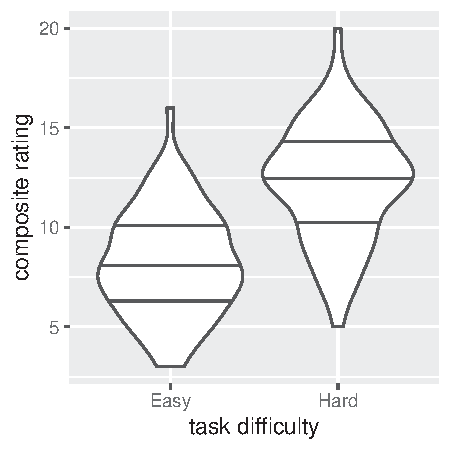
\includegraphics[width=.5\linewidth]{figure/graphics-gg_subjectRating-show-1} 

}



\end{knitrout}
\caption{Violin plots of the effort + difficulty + frustration ratings, as a function of task difficulty.}\label{fig:eTaskTaring.Violin}
\end{figure}

\paragraph{Effect of task difficulty on false-alarm rate} (\Cref{fig:eTaskFA.Violin})

\begin{knitrout}\footnotesize
\definecolor{shadecolor}{rgb}{0.969, 0.969, 0.969}\color{fgcolor}\begin{kframe}
\begin{alltt}
\hlstd{eTaskSubFA} \hlkwb{<-} \hlstd{eTaskSub} \hlopt
  \hlkwd{filter}\hlstd{(sigDet} \hlopt{==} \hlstr{"FA"}\hlstd{)}
\hlkwd{ggplot}\hlstd{(}
  \hlkwc{data} \hlstd{= eTaskSubFA,}
  \hlkwd{aes}\hlstd{(}
    \hlkwc{x} \hlstd{= taskDifficulty,}
    \hlkwc{y} \hlstd{= prop,}
    \hlkwc{group} \hlstd{= taskDifficulty}
  \hlstd{)}
\hlstd{)} \hlopt{+}
  \hlkwd{geom_violin}\hlstd{(}\hlkwc{draw_quantiles} \hlstd{=} \hlkwd{c}\hlstd{(}\hlnum{0.25}\hlstd{,} \hlnum{0.5}\hlstd{,} \hlnum{0.75}\hlstd{))} \hlopt{+}
  \hlkwd{labs}\hlstd{(}\hlkwc{x} \hlstd{=} \hlstr{"task difficulty"}\hlstd{,} \hlkwc{y} \hlstd{=} \hlstr{"false-alarm rate"}\hlstd{)}
\end{alltt}
\end{kframe}
\end{knitrout}

\begin{figure}
\begin{knitrout}\footnotesize
\definecolor{shadecolor}{rgb}{0.969, 0.969, 0.969}\color{fgcolor}

{\centering 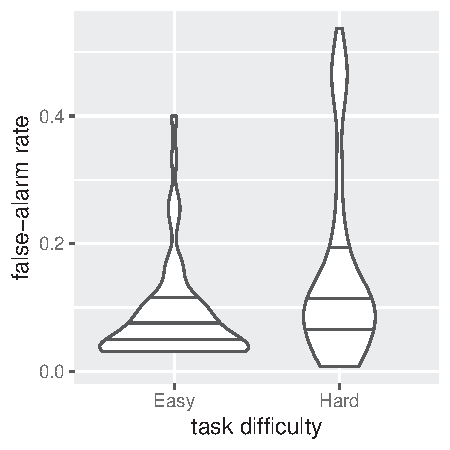
\includegraphics[width=.5\linewidth]{figure/graphics-gg_subjectProp-show-1} 

}



\end{knitrout}
\caption{Violin plots of the false-alarm rate, as a function of task difficulty.}\label{fig:eTaskFA.Violin}
\end{figure}

\paragraph{Effect of task difficulty on RT} (\Cref{fig:eTaskRT.Violin})

\begin{knitrout}\footnotesize
\definecolor{shadecolor}{rgb}{0.969, 0.969, 0.969}\color{fgcolor}\begin{kframe}
\begin{alltt}
\hlkwd{ggplot}\hlstd{(}
  \hlkwc{data} \hlstd{= eTaskSub,}
  \hlkwd{aes}\hlstd{(}
    \hlkwc{x} \hlstd{= taskDifficulty,}
    \hlkwc{y} \hlstd{= geomMean.eTask.RT,}
    \hlkwc{color} \hlstd{= sigDet}
  \hlstd{)}
\hlstd{)} \hlopt{+}
  \hlkwd{geom_violin}\hlstd{(}\hlkwc{draw_quantiles} \hlstd{=} \hlkwd{c}\hlstd{(}\hlnum{0.25}\hlstd{,} \hlnum{0.5}\hlstd{,} \hlnum{0.75}\hlstd{))} \hlopt{+}
  \hlkwd{labs}\hlstd{(}\hlkwc{x} \hlstd{=} \hlstr{"task difficulty"}\hlstd{,} \hlkwc{y} \hlstd{=} \hlstr{"RT (geometric mean)"}\hlstd{)} \hlopt{+}
  \hlkwd{theme}\hlstd{(}
    \hlkwc{legend.position} \hlstd{=} \hlkwd{c}\hlstd{(}\hlnum{0.05}\hlstd{,} \hlnum{0.95}\hlstd{),}
    \hlkwc{legend.justification} \hlstd{=} \hlkwd{c}\hlstd{(}\hlnum{0.05}\hlstd{,} \hlnum{0.95}\hlstd{)}
  \hlstd{)}
\end{alltt}
\end{kframe}
\end{knitrout}

\begin{figure}
\begin{knitrout}\footnotesize
\definecolor{shadecolor}{rgb}{0.969, 0.969, 0.969}\color{fgcolor}

{\centering 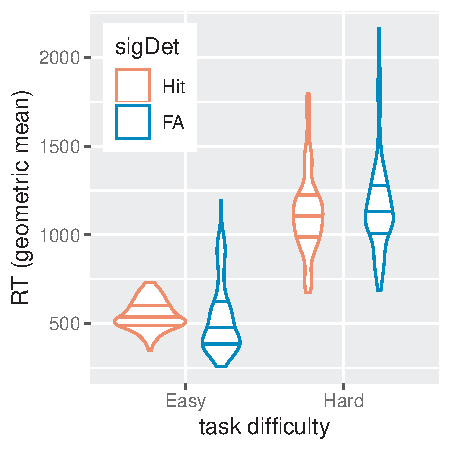
\includegraphics[width=.5\linewidth]{figure/graphics-gg_subjectRT-show-1} 

}



\end{knitrout}
\caption{Violin plots of geometric mean RT, as a function of task difficulty and signal detection.}\label{fig:eTaskRT.Violin}
\end{figure}

\subsection{MSIT task data}

\subsubsection{Disregarding subjects}

\paragraph{RT} Transform RT?

\begin{knitrout}\footnotesize
\definecolor{shadecolor}{rgb}{0.969, 0.969, 0.969}\color{fgcolor}\begin{kframe}
\begin{alltt}
\hlstd{lmMTask} \hlkwb{<-} \hlkwd{lm}\hlstd{(reactionTime} \hlopt{~} \hlstd{sigDet} \hlopt{*} \hlstd{trialType,} \hlkwc{data} \hlstd{= mTask)}
\end{alltt}
\end{kframe}
\end{knitrout}

\begin{knitrout}\footnotesize
\definecolor{shadecolor}{rgb}{0.969, 0.969, 0.969}\color{fgcolor}\begin{kframe}
\begin{alltt}
\hlstd{lambda.mTask} \hlkwb{<-} \hlkwd{powerTransform}\hlstd{(lmMTask)} \hlopt
  \hlkwd{print}\hlstd{()}
\end{alltt}
\begin{verbatim}
Estimated transformation parameter 
         Y1 
-0.05513577 
\end{verbatim}
\end{kframe}
\end{knitrout}

\noindent We should transform \code{reactionTime} because $\lambda = -0.06 \approx 0$. We also show this graphically in \Cref{fig:mTaskBoxCox}:

\begin{knitrout}\footnotesize
\definecolor{shadecolor}{rgb}{0.969, 0.969, 0.969}\color{fgcolor}\begin{kframe}
\begin{alltt}
\hlkwd{gg_boxcox}\hlstd{(lmMTask)}
\end{alltt}
\end{kframe}
\end{knitrout}

\begin{figure}
\begin{knitrout}\footnotesize
\definecolor{shadecolor}{rgb}{0.969, 0.969, 0.969}\color{fgcolor}

{\centering 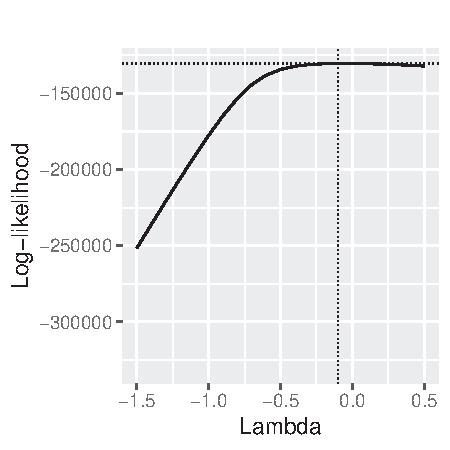
\includegraphics[width=.5\linewidth]{figure/graphics-lm_mTask_boxcox_show-1} 

}



\end{knitrout}
\caption{Plot profile log-likelihoods for the parameter of the Box-Cox power family for \code{lmMTask}.}\label{fig:mTaskBoxCox}
\end{figure}

Transform RT, and compare models.

\begin{knitrout}\footnotesize
\definecolor{shadecolor}{rgb}{0.969, 0.969, 0.969}\color{fgcolor}\begin{kframe}
\begin{alltt}
\hlstd{mTask} \hlkwb{<-} \hlstd{mTask} \hlopt
  \hlkwd{mutate}\hlstd{(}\hlkwc{reactionTimeLog} \hlstd{=} \hlkwd{log}\hlstd{(reactionTime))}
\hlstd{lmMTaskLog} \hlkwb{<-} \hlkwd{lm}\hlstd{(reactionTimeLog} \hlopt{~} \hlstd{sigDet} \hlopt{*} \hlstd{trialType,} \hlkwc{data} \hlstd{= mTask)}
\hlkwd{AIC}\hlstd{(lmMTask, lmMTaskLog)} \hlopt
  \hlkwd{as_tibble}\hlstd{()} \hlopt
  \hlkwd{kable}\hlstd{(}\hlkwc{digits} \hlstd{=} \hlnum{0}\hlstd{,} \hlkwc{booktabs} \hlstd{=} \hlnum{TRUE}\hlstd{)} \hlopt
  \hlkwd{kable_styling}\hlstd{(}\hlkwc{position} \hlstd{=} \hlstr{"center"}\hlstd{)}
\end{alltt}
\end{kframe}\begin{table}[H]
\centering
\begin{tabular}{rr}
\toprule
df & AIC\\
\midrule
7 & 449639\\
7 & 13896\\
\bottomrule
\end{tabular}
\end{table}


\end{knitrout}

Here too, there is no doubt that taking the log is the right thing to do.

\paragraph{Measures of accuracy}

Measures of association for ordinal factors (\code{stimulus}, \code{response}) in a two-way table:

\begin{knitrout}\footnotesize
\definecolor{shadecolor}{rgb}{0.969, 0.969, 0.969}\color{fgcolor}\begin{kframe}
\begin{alltt}
\hlstd{mTaskTab} \hlkwb{<-} \hlkwd{with}\hlstd{(mTask,} \hlkwd{table}\hlstd{(response, stimulus))}
\hlkwd{library}\hlstd{(questionr)}
\hlstd{cv} \hlkwb{<-} \hlkwd{cramer.v}\hlstd{(mTaskTab)}
\hlkwd{library}\hlstd{(DescTools)}
\hlstd{gkg} \hlkwb{<-} \hlkwd{GoodmanKruskalGamma}\hlstd{(mTaskTab)}
\hlstd{gkt} \hlkwb{<-} \hlkwd{GoodmanKruskalTau}\hlstd{(mTaskTab)}
\hlstd{l} \hlkwb{<-} \hlkwd{Lambda}\hlstd{(mTaskTab)}
\hlkwd{tribble}\hlstd{(}
  \hlopt{~}\hlstd{measure,} \hlopt{~}\hlstd{value,}
  \hlstr{"Cramer's V"}\hlstd{, cv,}
  \hlstr{"Goodman-Kruskal Gamma"}\hlstd{, gkg,}
  \hlstr{"Goodman-Kruskal Tau"}\hlstd{, gkt,}
  \hlstr{"Lambda"}\hlstd{, l}
\hlstd{)} \hlopt
  \hlkwd{kable}\hlstd{(}\hlkwc{digits} \hlstd{=} \hlnum{2}\hlstd{,} \hlkwc{booktabs} \hlstd{=} \hlnum{TRUE}\hlstd{)} \hlopt
  \hlkwd{kable_styling}\hlstd{(}\hlkwc{position} \hlstd{=} \hlstr{"center"}\hlstd{)}
\end{alltt}
\end{kframe}\begin{table}[H]
\centering
\begin{tabular}{lr}
\toprule
measure & value\\
\midrule
Cramer's V & 0.82\\
Goodman-Kruskal Gamma & 0.92\\
Goodman-Kruskal Tau & 0.67\\
Lambda & 0.81\\
\bottomrule
\end{tabular}
\end{table}


\end{knitrout}

\noindent These measures represent how well the subjects responded to each stimulus with the corresponding correct response.

Using \emph{Lambda} (as an example) we summarize accuracy as a function of trial type and signal detection category:

\begin{knitrout}\footnotesize
\definecolor{shadecolor}{rgb}{0.969, 0.969, 0.969}\color{fgcolor}\begin{kframe}
\begin{alltt}
\hlkwd{library}\hlstd{(questionr)}
\hlstd{mTaskC} \hlkwb{<-} \hlstd{mTask} \hlopt
  \hlkwd{filter}\hlstd{(trialType} \hlopt{==} \hlstr{"Congruent"}\hlstd{)} \hlopt
  \hlkwd{select}\hlstd{(stimulus, response)} \hlopt
  \hlkwd{table}\hlstd{()} \hlopt
  \hlkwd{cramer.v}\hlstd{()} \hlopt
  \hlkwd{print}\hlstd{()}
\end{alltt}
\begin{verbatim}
[1] 0.9823959
\end{verbatim}
\begin{alltt}
\hlstd{mTaskI} \hlkwb{<-} \hlstd{mTask} \hlopt
  \hlkwd{filter}\hlstd{(trialType} \hlopt{==} \hlstr{"Incongruent"}\hlstd{)} \hlopt
  \hlkwd{select}\hlstd{(stimulus, response)} \hlopt
  \hlkwd{table}\hlstd{()} \hlopt
  \hlkwd{cramer.v}\hlstd{()} \hlopt
  \hlkwd{print}\hlstd{()}
\end{alltt}
\begin{verbatim}
[1] 0.6559378
\end{verbatim}
\end{kframe}
\end{knitrout}
\begin{knitrout}\footnotesize
\definecolor{shadecolor}{rgb}{0.969, 0.969, 0.969}\color{fgcolor}\begin{kframe}
\begin{alltt}
\hlstd{mTaskCramerS} \hlkwb{<-} \hlstd{mTask} \hlopt
  \hlkwd{group_by}\hlstd{(trialType, subject)} \hlopt
  \hlkwd{nest}\hlstd{()} \hlopt
  \hlkwd{mutate}\hlstd{(}\hlkwc{cv} \hlstd{=} \hlkwd{map}\hlstd{(data,} \hlopt{~}
  \hlkwd{select}\hlstd{(.x,} \hlkwd{c}\hlstd{(stimulus, response))} \hlopt
    \hlkwd{table}\hlstd{()} \hlopt
    \hlkwd{cramer.v}\hlstd{()} \hlopt
    \hlkwd{as.list}\hlstd{()} \hlopt
    \hlkwd{as_tibble}\hlstd{(}\hlkwc{.name_repair} \hlstd{=} \hlopt{~} \hlkwd{c}\hlstd{(}\hlstr{"Cramer_V"}\hlstd{))))} \hlopt
  \hlkwd{select}\hlstd{(}\hlopt{-}\hlstd{data)} \hlopt
  \hlkwd{unnest}\hlstd{(cv)} \hlopt
  \hlkwd{ungroup}\hlstd{()}
\hlkwd{glimpse}\hlstd{(mTaskCramerS)}
\end{alltt}
\begin{verbatim}
Observations: 330
Variables: 3
$ subject   <fct> 1, 1, 10, 10, 100, 100, 101, 101, 102, 102, 103, 103, 104...
$ trialType <fct> Congruent, Incongruent, Congruent, Incongruent, Congruent...
$ Cramer_V  <dbl> 0.98373875, 0.38283932, 1.00000000, 0.72519159, 1.0000000...
\end{verbatim}
\end{kframe}
\end{knitrout}

\paragraph{Effect of trial type on accuracy} (\Cref{fig:mTaskCramerS})
  
\begin{knitrout}\footnotesize
\definecolor{shadecolor}{rgb}{0.969, 0.969, 0.969}\color{fgcolor}\begin{kframe}
\begin{alltt}
\hlstd{mTaskCramerS} \hlkwb{<-} \hlstd{mTaskCramerS} \hlopt
  \hlkwd{spread}\hlstd{(}\hlkwc{key} \hlstd{= trialType,} \hlkwc{value} \hlstd{= Cramer_V)} \hlopt
  \hlkwd{mutate}\hlstd{(}\hlkwc{diff} \hlstd{= Congruent} \hlopt{-} \hlstd{Incongruent)}
\hlstd{mTaskDiff} \hlkwb{<-} \hlkwd{tibble}\hlstd{(}\hlkwc{bySubject} \hlstd{= mTaskCramerS}\hlopt{$}\hlstd{diff)}
\hlkwd{ggplot}\hlstd{(}\hlkwc{data} \hlstd{= mTaskDiff,} \hlkwd{aes}\hlstd{(}
  \hlkwc{x} \hlstd{=} \hlstr{""}\hlstd{,}
  \hlkwc{y} \hlstd{= bySubject}
\hlstd{))} \hlopt{+}
  \hlkwd{geom_violin}\hlstd{(}\hlkwc{draw_quantiles} \hlstd{=} \hlkwd{c}\hlstd{(}\hlnum{0.25}\hlstd{,} \hlnum{0.5}\hlstd{,} \hlnum{0.75}\hlstd{))} \hlopt{+}
  \hlkwd{labs}\hlstd{(}\hlkwc{x} \hlstd{=} \hlstr{""}\hlstd{,} \hlkwc{y} \hlstd{=} \hlstr{"difference in Cramer's V"}\hlstd{)}
\end{alltt}
\end{kframe}
\end{knitrout}

\begin{figure}
\begin{knitrout}\footnotesize
\definecolor{shadecolor}{rgb}{0.969, 0.969, 0.969}\color{fgcolor}

{\centering 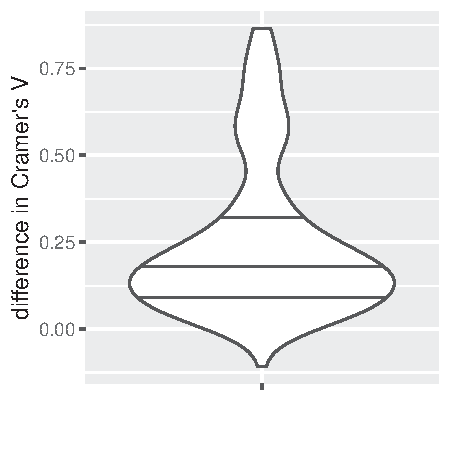
\includegraphics[width=.5\linewidth]{figure/graphics-gg_mTaskCramerS-show-1} 

}



\end{knitrout}
\caption{Violin plots of the difference between Cramer's V for congruent and incongruent trials.}\label{fig:mTaskCramerS}
\end{figure}

\noindent The median difference between Cramer's V for congruent and incongruent trials is 0.18.

\subsubsection{Join tibbles}

\begin{knitrout}\footnotesize
\definecolor{shadecolor}{rgb}{0.969, 0.969, 0.969}\color{fgcolor}\begin{kframe}
\begin{alltt}
\hlstd{eTaskmTaskSub} \hlkwb{<-} \hlstd{eTaskSub} \hlopt
  \hlkwd{full_join}\hlstd{(mTaskCramerS)}
\hlkwd{dim}\hlstd{(eTaskmTaskSub)}
\end{alltt}
\begin{verbatim}
[1] 305  15
\end{verbatim}
\begin{alltt}
\hlstd{eTaskSub} \hlkwb{<-} \hlstd{eTaskSub} \hlopt
  \hlkwd{drop_na}\hlstd{()}
\hlkwd{dim}\hlstd{(eTaskmTaskSub)}
\end{alltt}
\begin{verbatim}
[1] 305  15
\end{verbatim}
\begin{alltt}
\hlkwd{glimpse}\hlstd{(eTaskmTaskSub)}
\end{alltt}
\begin{verbatim}
Observations: 305
Variables: 15
$ taskDifficulty    <fct> Easy, Easy, Easy, Easy, Easy, Easy, Easy, Easy, E...
$ gender            <fct> Female, Female, Male, Female, Female, Female, Fem...
$ subject           <fct> 1, 1, 2, 3, 3, 5, 5, 6, 8, 8, 9, 9, 10, 10, 11, 1...
$ effortRating      <dbl> 2, 2, 5, 5, 5, 2, 2, 3, 2, 2, 2, 2, 4, 4, 2, 2, 2...
$ difficultyRating  <dbl> 1, 1, 3, 1, 1, 3, 3, 2, 2, 2, 3, 3, 3, 3, 4, 4, 2...
$ frustrationRating <dbl> 1, 1, 2, 1, 1, 1, 1, 1, 2, 2, 1, 1, 1, 1, 3, 3, 4...
$ fatigueRating     <dbl> 6, 6, 4, 2, 2, 5, 5, 3, 3, 3, 5, 5, 2, 2, 2, 2, 6...
$ signalNoise       <fct> Signal, Noise, Signal, Signal, Noise, Signal, Noi...
$ sigDet            <fct> Hit, FA, Hit, Hit, FA, Hit, FA, Hit, Hit, FA, Hit...
$ prop              <dbl> 1.00000000, 0.03225806, 1.00000000, 1.00000000, 0...
$ geomMean.eTask.RT <dbl> 520.2102, 488.0000, 572.2292, 514.5156, 398.8283,...
$ rating            <dbl> 4, 4, 10, 7, 7, 6, 6, 6, 6, 6, 6, 6, 8, 8, 9, 9, ...
$ Congruent         <dbl> 0.9837388, 0.9837388, 0.9856697, 1.0000000, 1.000...
$ Incongruent       <dbl> 0.3828393, 0.3828393, 0.8083788, 0.7994993, 0.799...
$ diff              <dbl> 0.6008994, 0.6008994, 0.1772909, 0.2005007, 0.200...
\end{verbatim}
\begin{alltt}
\hlstd{eTaskmTaskSubT} \hlkwb{<-} \hlstd{eTaskmTaskSub} \hlopt
  \hlkwd{gather}\hlstd{(congruence, CramerV, Congruent}\hlopt{:}\hlstd{Incongruent,} \hlkwc{factor_key} \hlstd{=} \hlnum{TRUE}\hlstd{)}
\hlkwd{glimpse}\hlstd{(eTaskmTaskSubT)}
\end{alltt}
\begin{verbatim}
Observations: 610
Variables: 15
$ taskDifficulty    <fct> Easy, Easy, Easy, Easy, Easy, Easy, Easy, Easy, E...
$ gender            <fct> Female, Female, Male, Female, Female, Female, Fem...
$ subject           <fct> 1, 1, 2, 3, 3, 5, 5, 6, 8, 8, 9, 9, 10, 10, 11, 1...
$ effortRating      <dbl> 2, 2, 5, 5, 5, 2, 2, 3, 2, 2, 2, 2, 4, 4, 2, 2, 2...
$ difficultyRating  <dbl> 1, 1, 3, 1, 1, 3, 3, 2, 2, 2, 3, 3, 3, 3, 4, 4, 2...
$ frustrationRating <dbl> 1, 1, 2, 1, 1, 1, 1, 1, 2, 2, 1, 1, 1, 1, 3, 3, 4...
$ fatigueRating     <dbl> 6, 6, 4, 2, 2, 5, 5, 3, 3, 3, 5, 5, 2, 2, 2, 2, 6...
$ signalNoise       <fct> Signal, Noise, Signal, Signal, Noise, Signal, Noi...
$ sigDet            <fct> Hit, FA, Hit, Hit, FA, Hit, FA, Hit, Hit, FA, Hit...
$ prop              <dbl> 1.00000000, 0.03225806, 1.00000000, 1.00000000, 0...
$ geomMean.eTask.RT <dbl> 520.2102, 488.0000, 572.2292, 514.5156, 398.8283,...
$ rating            <dbl> 4, 4, 10, 7, 7, 6, 6, 6, 6, 6, 6, 6, 8, 8, 9, 9, ...
$ diff              <dbl> 0.6008994, 0.6008994, 0.1772909, 0.2005007, 0.200...
$ congruence        <fct> Congruent, Congruent, Congruent, Congruent, Congr...
$ CramerV           <dbl> 0.9837388, 0.9837388, 0.9856697, 1.0000000, 1.000...
\end{verbatim}
\begin{alltt}
\hlstd{eTaskmTaskSubT} \hlopt
  \hlkwd{count}\hlstd{(taskDifficulty)} \hlopt
  \hlkwd{mutate}\hlstd{(}\hlkwc{prop} \hlstd{=} \hlkwd{prop.table}\hlstd{(n))} \hlopt
  \hlkwd{mkable}\hlstd{()}
\end{alltt}


{\ttfamily\noindent\color{warningcolor}{Warning: Factor `taskDifficulty` contains implicit NA, consider using `forcats::fct\_explicit\_na`}}\end{kframe}\begin{table}[H]
\centering
\begin{tabular}{lrr}
\toprule
taskDifficulty & n & prop\\
\midrule
Easy & 278 & 0.46\\
Hard & 326 & 0.53\\
NA & 6 & 0.01\\
\bottomrule
\end{tabular}
\end{table}

\begin{kframe}\begin{alltt}
\hlstd{eTaskmTaskSubT} \hlkwb{<-} \hlstd{eTaskmTaskSubT} \hlopt
  \hlkwd{drop_na}\hlstd{()}
\hlstd{eTaskmTaskSubT} \hlopt
  \hlkwd{count}\hlstd{(taskDifficulty)} \hlopt
  \hlkwd{mutate}\hlstd{(}\hlkwc{prop} \hlstd{=} \hlkwd{prop.table}\hlstd{(n))} \hlopt
  \hlkwd{mkable}\hlstd{()}
\end{alltt}
\end{kframe}\begin{table}[H]
\centering
\begin{tabular}{lrr}
\toprule
taskDifficulty & n & prop\\
\midrule
Easy & 278 & 0.46\\
Hard & 326 & 0.54\\
\bottomrule
\end{tabular}
\end{table}


\end{knitrout}

\begin{knitrout}\footnotesize
\definecolor{shadecolor}{rgb}{0.969, 0.969, 0.969}\color{fgcolor}\begin{kframe}
\begin{alltt}
\hlkwd{ggplot}\hlstd{(}\hlkwc{data} \hlstd{= eTaskmTaskSubT,} \hlkwd{aes}\hlstd{(}
  \hlkwc{x} \hlstd{= taskDifficulty,}
  \hlkwc{y} \hlstd{= CramerV,} \hlkwc{color} \hlstd{= congruence}
\hlstd{))} \hlopt{+}
  \hlkwd{geom_boxplot}\hlstd{()} \hlopt{+}
  \hlkwd{labs}\hlstd{(}\hlkwc{x} \hlstd{=} \hlstr{"task difficulty"}\hlstd{,} \hlkwc{y} \hlstd{=} \hlstr{"Cramer's V"}\hlstd{)}
\end{alltt}
\end{kframe}
\end{knitrout}

\begin{figure}
\begin{knitrout}\footnotesize
\definecolor{shadecolor}{rgb}{0.969, 0.969, 0.969}\color{fgcolor}

{\centering 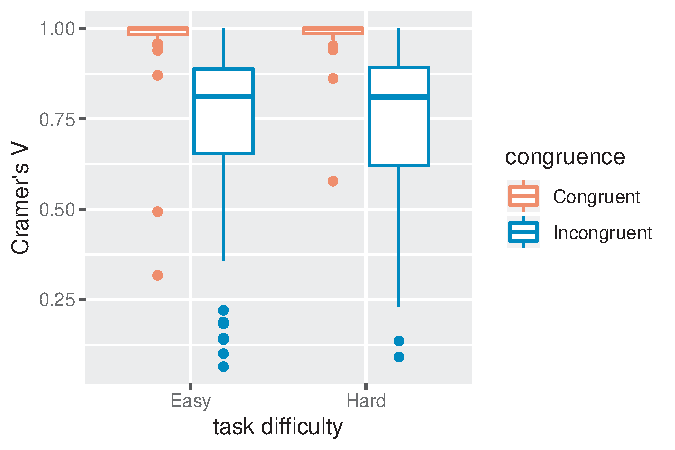
\includegraphics[width=0.75\linewidth]{figure/graphics-gg_eTaskmTaskSub-show-1} 

}



\end{knitrout}
\caption{Boxplots of Cramer's V as a function of \code{e} task difficulty and congruence in the MSIT task.}\label{fig:eTaskmTaskSub}
\end{figure}

\begin{knitrout}\footnotesize
\definecolor{shadecolor}{rgb}{0.969, 0.969, 0.969}\color{fgcolor}\begin{kframe}
\begin{alltt}
\hlkwd{ggplot}\hlstd{(}\hlkwc{data} \hlstd{= eTaskmTaskSubT,} \hlkwd{aes}\hlstd{(}
  \hlkwc{x} \hlstd{= rating,}
  \hlkwc{y} \hlstd{= CramerV,} \hlkwc{color} \hlstd{= congruence}
\hlstd{))} \hlopt{+}
  \hlkwd{geom_point}\hlstd{()} \hlopt{+}
  \hlkwd{labs}\hlstd{(}\hlkwc{x} \hlstd{=} \hlstr{"rating"}\hlstd{,} \hlkwc{y} \hlstd{=} \hlstr{"Cramer's V"}\hlstd{)}
\end{alltt}
\end{kframe}
\end{knitrout}

\begin{figure}
\begin{knitrout}\footnotesize
\definecolor{shadecolor}{rgb}{0.969, 0.969, 0.969}\color{fgcolor}

{\centering 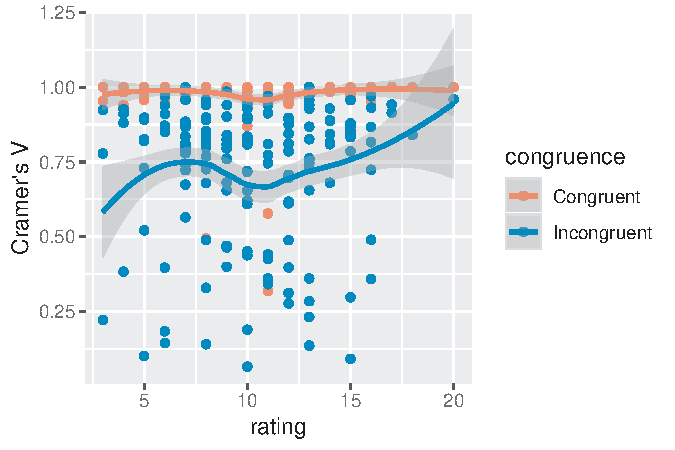
\includegraphics[width=0.75\linewidth]{figure/graphics-gg_eTaskRatingmTaskCong-show-1} 

}



\end{knitrout}
\caption{Cramer's V as a function of \code{e} rating and congruence in the MSIT task.}\label{fig:eTaskmTaskSub}
\end{figure}

\begin{knitrout}\footnotesize
\definecolor{shadecolor}{rgb}{0.969, 0.969, 0.969}\color{fgcolor}\begin{kframe}
\begin{alltt}
\hlstd{all} \hlkwb{<-} \hlstd{eTaskmTaskSub} \hlopt
  \hlkwd{full_join}\hlstd{(mTask)}
\end{alltt}


{\ttfamily\noindent\color{warningcolor}{Warning: Column `sigDet` joining factors with different levels, coercing to character vector}}\begin{alltt}
\hlkwd{dim}\hlstd{(all)}
\end{alltt}
\begin{verbatim}
[1] 33143    20
\end{verbatim}
\begin{alltt}
\hlstd{all} \hlkwb{<-} \hlstd{all} \hlopt
  \hlkwd{drop_na}\hlstd{()}
\hlkwd{dim}\hlstd{(all)}
\end{alltt}
\begin{verbatim}
[1] 28219    20
\end{verbatim}
\begin{alltt}
\hlkwd{glimpse}\hlstd{(all)}
\end{alltt}
\begin{verbatim}
Observations: 28,219
Variables: 20
$ taskDifficulty    <fct> Easy, Easy, Easy, Easy, Easy, Easy, Easy, Easy, E...
$ gender            <fct> Female, Female, Female, Female, Female, Female, F...
$ subject           <fct> 1, 1, 1, 1, 1, 1, 1, 1, 1, 1, 1, 1, 1, 1, 1, 1, 1...
$ effortRating      <dbl> 2, 2, 2, 2, 2, 2, 2, 2, 2, 2, 2, 2, 2, 2, 2, 2, 2...
$ difficultyRating  <dbl> 1, 1, 1, 1, 1, 1, 1, 1, 1, 1, 1, 1, 1, 1, 1, 1, 1...
$ frustrationRating <dbl> 1, 1, 1, 1, 1, 1, 1, 1, 1, 1, 1, 1, 1, 1, 1, 1, 1...
$ fatigueRating     <dbl> 6, 6, 6, 6, 6, 6, 6, 6, 6, 6, 6, 6, 6, 6, 6, 6, 6...
$ signalNoise       <fct> Signal, Signal, Signal, Signal, Signal, Signal, S...
$ sigDet            <chr> "Hit", "Hit", "Hit", "Hit", "Hit", "Hit", "Hit", ...
$ prop              <dbl> 1, 1, 1, 1, 1, 1, 1, 1, 1, 1, 1, 1, 1, 1, 1, 1, 1...
$ geomMean.eTask.RT <dbl> 520.2102, 520.2102, 520.2102, 520.2102, 520.2102,...
$ rating            <dbl> 4, 4, 4, 4, 4, 4, 4, 4, 4, 4, 4, 4, 4, 4, 4, 4, 4...
$ Congruent         <dbl> 0.9837388, 0.9837388, 0.9837388, 0.9837388, 0.983...
$ Incongruent       <dbl> 0.3828393, 0.3828393, 0.3828393, 0.3828393, 0.382...
$ diff              <dbl> 0.6008994, 0.6008994, 0.6008994, 0.6008994, 0.600...
$ response          <int> 1, 3, 3, 1, 3, 2, 3, 1, 1, 2, 3, 1, 2, 2, 1, 3, 1...
$ stimulus          <int> 1, 3, 3, 1, 3, 2, 3, 1, 1, 2, 3, 1, 2, 2, 1, 3, 1...
$ reactionTime      <int> 530, 538, 489, 529, 553, 593, 457, 417, 449, 762,...
$ trialType         <fct> Congruent, Congruent, Congruent, Congruent, Congr...
$ reactionTimeLog   <dbl> 6.272877, 6.287859, 6.192362, 6.270988, 6.315358,...
\end{verbatim}
\end{kframe}
\end{knitrout}

\begin{knitrout}\footnotesize
\definecolor{shadecolor}{rgb}{0.969, 0.969, 0.969}\color{fgcolor}\begin{kframe}
\begin{alltt}
\hlkwd{ggplot}\hlstd{(}\hlkwc{data} \hlstd{= all,} \hlkwd{aes}\hlstd{(}
  \hlkwc{x} \hlstd{= taskDifficulty,}
  \hlkwc{y} \hlstd{= reactionTimeLog,} \hlkwc{color} \hlstd{= trialType}
\hlstd{))} \hlopt{+}
  \hlkwd{geom_violin}\hlstd{()} \hlopt{+}
  \hlkwd{labs}\hlstd{(}\hlkwc{x} \hlstd{=} \hlstr{"e task difficult"}\hlstd{,} \hlkwc{y} \hlstd{=} \hlstr{"m task log(RT)"}\hlstd{)}
\end{alltt}
\end{kframe}
\end{knitrout}

\begin{figure}
\begin{knitrout}\footnotesize
\definecolor{shadecolor}{rgb}{0.969, 0.969, 0.969}\color{fgcolor}

{\centering 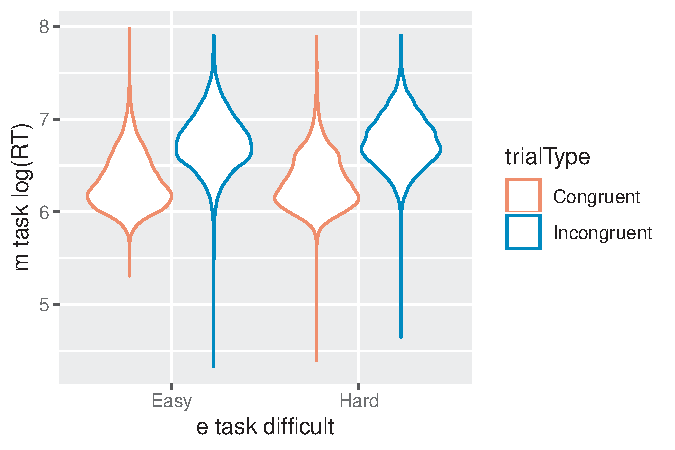
\includegraphics[width=0.75\linewidth]{figure/graphics-gg_all-show-1} 

}



\end{knitrout}
\caption{Log(RT) as a function of \code{e} task difficulty and congruence in the MSIT task.}\label{fig:eTaskmTaskSub}
\end{figure}


\subsection{Linear mixed-effects model}

\begin{knitrout}\footnotesize
\definecolor{shadecolor}{rgb}{0.969, 0.969, 0.969}\color{fgcolor}\begin{kframe}
\begin{alltt}
\hlstd{lmeMTaskLog} \hlkwb{<-}
  \hlkwd{lmer}\hlstd{(reactionTimeLog} \hlopt{~} \hlstd{sigDet} \hlopt{*} \hlstd{trialType} \hlopt{+}
    \hlstd{(}\hlnum{1} \hlopt{|} \hlstd{subject),} \hlkwc{data} \hlstd{= mTask)}
\end{alltt}
\end{kframe}
\end{knitrout}

More complex random effects

\begin{knitrout}\footnotesize
\definecolor{shadecolor}{rgb}{0.969, 0.969, 0.969}\color{fgcolor}\begin{kframe}
\begin{alltt}
\hlstd{lmeMTaskLog2} \hlkwb{<-}
  \hlkwd{lmer}\hlstd{(reactionTimeLog} \hlopt{~} \hlstd{sigDet} \hlopt{*} \hlstd{trialType} \hlopt{+}
    \hlstd{(sigDet} \hlopt{*} \hlstd{trialType} \hlopt{|} \hlstd{subject),}
  \hlkwc{data} \hlstd{= mTask}
  \hlstd{)}
\end{alltt}


{\ttfamily\noindent\color{warningcolor}{Warning in checkConv(attr(opt, "{}derivs"{}), opt\$par, ctrl = control\$checkConv, : Model failed to converge with max|grad| = 0.117414 (tol = 0.002, component 1)}}\begin{alltt}
\hlkwd{AIC}\hlstd{(lmeMTaskLog, lmeMTaskLog2)} \hlopt
  \hlkwd{as_tibble}\hlstd{()} \hlopt
  \hlkwd{kable}\hlstd{(}\hlkwc{digits} \hlstd{=} \hlnum{0}\hlstd{,} \hlkwc{booktabs} \hlstd{=} \hlnum{TRUE}\hlstd{)} \hlopt
  \hlkwd{kable_styling}\hlstd{(}\hlkwc{position} \hlstd{=} \hlstr{"center"}\hlstd{)}
\end{alltt}
\end{kframe}\begin{table}[H]
\centering
\begin{tabular}{rr}
\toprule
df & AIC\\
\midrule
8 & 131\\
28 & -1814\\
\bottomrule
\end{tabular}
\end{table}


\end{knitrout}

\begin{knitrout}\footnotesize
\definecolor{shadecolor}{rgb}{0.969, 0.969, 0.969}\color{fgcolor}\begin{kframe}
\begin{alltt}
\hlkwd{tidy}\hlstd{(lmeMTaskLog2,} \hlkwc{effects} \hlstd{=} \hlstr{"ran_pars"}\hlstd{)} \hlopt
  \hlkwd{mkables}\hlstd{()}
\end{alltt}
\end{kframe}\begin{table}[H]
\centering
\resizebox{\linewidth}{!}{
\begin{tabular}{lllr}
\toprule
effect & group & term & estimate\\
\midrule
ran\_pars & subject & sd\_\_(Intercept) & 0.19\\
ran\_pars & subject & sd\_\_sigDetFA2 & 0.13\\
ran\_pars & subject & sd\_\_sigDetFA1 & 0.33\\
ran\_pars & subject & sd\_\_trialTypeIncongruent & 0.13\\
ran\_pars & subject & sd\_\_sigDetFA2:trialTypeIncongruent & 0.27\\
\addlinespace
ran\_pars & subject & sd\_\_sigDetFA1:trialTypeIncongruent & 0.33\\
ran\_pars & subject & cor\_\_(Intercept).sigDetFA2 & 0.40\\
ran\_pars & subject & cor\_\_(Intercept).sigDetFA1 & 0.18\\
ran\_pars & subject & cor\_\_(Intercept).trialTypeIncongruent & -0.16\\
ran\_pars & subject & cor\_\_(Intercept).sigDetFA2:trialTypeIncongruent & -0.12\\
\addlinespace
ran\_pars & subject & cor\_\_(Intercept).sigDetFA1:trialTypeIncongruent & -0.14\\
ran\_pars & subject & cor\_\_sigDetFA2.sigDetFA1 & 0.05\\
ran\_pars & subject & cor\_\_sigDetFA2.trialTypeIncongruent & 0.52\\
ran\_pars & subject & cor\_\_sigDetFA2.sigDetFA2:trialTypeIncongruent & -0.19\\
ran\_pars & subject & cor\_\_sigDetFA2.sigDetFA1:trialTypeIncongruent & 0.08\\
\addlinespace
ran\_pars & subject & cor\_\_sigDetFA1.trialTypeIncongruent & -0.14\\
ran\_pars & subject & cor\_\_sigDetFA1.sigDetFA2:trialTypeIncongruent & 0.14\\
ran\_pars & subject & cor\_\_sigDetFA1.sigDetFA1:trialTypeIncongruent & -0.93\\
ran\_pars & subject & cor\_\_trialTypeIncongruent.sigDetFA2:trialTypeIncongruent & -0.61\\
ran\_pars & subject & cor\_\_trialTypeIncongruent.sigDetFA1:trialTypeIncongruent & -0.02\\
\addlinespace
ran\_pars & subject & cor\_\_sigDetFA2:trialTypeIncongruent.sigDetFA1:trialTypeIncongruent & -0.05\\
ran\_pars & Residual & sd\_\_Observation & 0.23\\
\bottomrule
\end{tabular}}
\end{table}


\end{knitrout}

\begin{knitrout}\footnotesize
\definecolor{shadecolor}{rgb}{0.969, 0.969, 0.969}\color{fgcolor}\begin{kframe}
\begin{alltt}
\hlkwd{library}\hlstd{(brms)}
\hlkwd{library}\hlstd{(dotwhisker)}
\hlkwd{tidy}\hlstd{(lmeMTaskLog2,} \hlkwc{effects} \hlstd{=} \hlstr{"fixed"}\hlstd{)} \hlopt
  \hlkwd{dwplot}\hlstd{(}\hlkwc{vline} \hlstd{=} \hlkwd{geom_vline}\hlstd{(}
    \hlkwc{xintercept} \hlstd{=} \hlnum{0}\hlstd{,}
    \hlkwc{colour} \hlstd{=} \hlstr{"grey50"}\hlstd{,}
    \hlkwc{linetype} \hlstd{=} \hlnum{2}
  \hlstd{))}
\end{alltt}
\end{kframe}
\end{knitrout}

\begin{figure}
\begin{knitrout}\footnotesize
\definecolor{shadecolor}{rgb}{0.969, 0.969, 0.969}\color{fgcolor}

{\centering 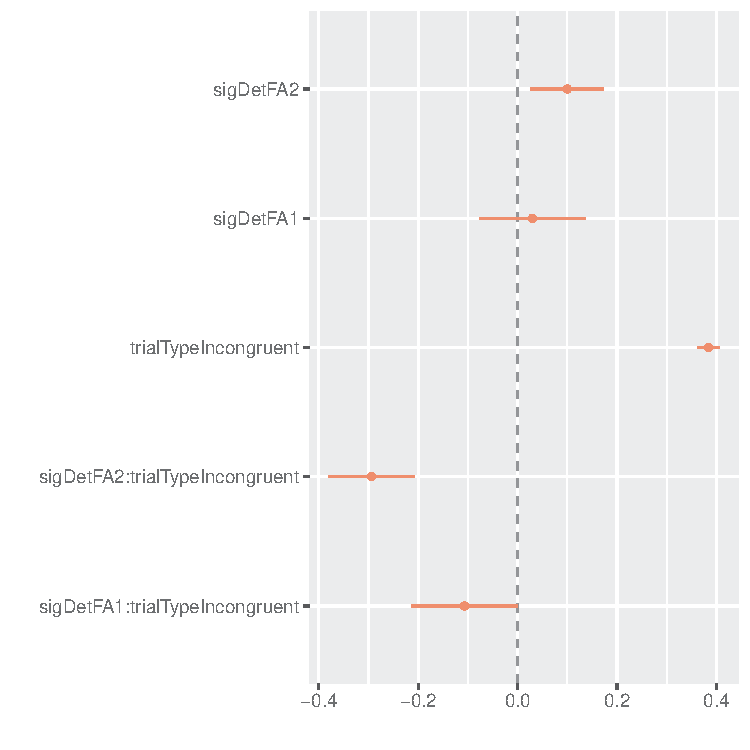
\includegraphics[width=\linewidth]{figure/graphics-lme_mTask_log_2_plot_show-1} 

}



\end{knitrout}
\caption{Dot-and-whisker plot of fixed effects of \code{lmeMTaskLog2} model .}\label{fig:lmeMTaskLog2plot}
\end{figure}
\pagebreak
\section*{R session information}

\begin{knitrout}\footnotesize
\definecolor{shadecolor}{rgb}{0.969, 0.969, 0.969}\color{fgcolor}\begin{kframe}
\begin{alltt}
\hlkwd{sessionInfo}\hlstd{()}
\end{alltt}
\begin{verbatim}
R version 3.6.1 (2019-07-05)
Platform: x86_64-apple-darwin15.6.0 (64-bit)
Running under: macOS Catalina 10.15.2

Matrix products: default
BLAS:   /Library/Frameworks/R.framework/Versions/3.6/Resources/lib/libRblas.0.dylib
LAPACK: /Library/Frameworks/R.framework/Versions/3.6/Resources/lib/libRlapack.dylib

locale:
[1] C

attached base packages:
[1] splines   parallel  stats     graphics  grDevices utils     datasets 
[8] methods   base     

other attached packages:
 [1] DescTools_0.99.31     questionr_0.7.0       janitor_1.2.0        
 [4] xtable_1.8-4          WWGbook_1.0.1         texreg_1.36.23       
 [7] styler_1.2.0          stargazer_5.2.2       R.utils_2.9.2        
[10] R.oo_1.23.0           R.methodsS3_1.7.1     qqplotr_0.0.3        
[13] prob_1.0-1            fAsianOptions_3042.82 fOptions_3042.86     
[16] fBasics_3042.89       timeSeries_3042.102   timeDate_3043.102    
[19] combinat_0.0-8        printr_0.1            predictmeans_1.0.1   
[22] mgcv_1.8-31           nlme_3.1-142          merTools_0.5.0       
[25] arm_1.10-1            MASS_7.3-51.4         lme4_1.1-21          
[28] Matrix_1.2-18         lintr_2.0.0           lindia_0.9           
[31] latex2exp_0.4.0       languageR_1.5.0       kableExtra_1.1.0     
[34] haven_2.2.0           gridExtra_2.3         ggfortify_0.4.8      
[37] formattable_0.2.0.1   foreign_0.8-72        foreach_1.4.7        
[40] extrafontdb_1.0       extrafont_0.17        effects_4.1-4        
[43] dotwhisker_0.5.0      car_3.0-5             carData_3.0-3        
[46] brms_2.10.0           Rcpp_1.0.3            broom.mixed_0.2.4    
[49] yardstick_0.0.4       rsample_0.0.5         recipes_0.1.7        
[52] parsnip_0.0.4         infer_0.5.1           dials_0.0.4          
[55] scales_1.1.0          broom_0.5.2           tidymodels_0.0.3     
[58] forcats_0.4.0         stringr_1.4.0         dplyr_0.8.3          
[61] purrr_0.3.3           readr_1.3.1           tidyr_1.0.0          
[64] tibble_2.1.3          ggplot2_3.2.1         tidyverse_1.3.0      
[67] knitr_1.26           

loaded via a namespace (and not attached):
  [1] SnowballC_0.6.0      coda_0.19-3          dygraphs_1.1.1.6    
  [4] data.table_1.12.6    rpart_4.1-15         inline_0.3.15       
  [7] generics_0.0.2       callr_3.3.2          future_1.15.1       
 [10] tokenizers_0.2.1     webshot_0.5.2        xml2_1.2.2          
 [13] lubridate_1.7.4      httpuv_1.5.2         StanHeaders_2.19.0  
 [16] assertthat_0.2.1     gower_0.2.1          xfun_0.11           
 [19] hms_0.5.2            bayesplot_1.7.1      evaluate_0.14       
 [22] promises_1.1.0       fansi_0.4.0          DEoptimR_1.0-8      
 [25] dbplyr_1.4.2         readxl_1.3.1         igraph_1.2.4.2      
 [28] DBI_1.0.0            htmlwidgets_1.5.1    stats4_3.6.1        
 [31] ellipsis_0.3.0       crosstalk_1.0.0      backports_1.1.5     
 [34] survey_3.36          markdown_1.1         vctrs_0.2.0         
 [37] remotes_2.1.0        abind_1.4-5          withr_2.1.2         
 [40] robustbase_0.93-5    xts_0.11-2           prettyunits_1.0.2   
 [43] cyclocomp_1.1.0      lazyeval_0.2.2       crayon_1.3.4        
 [46] labeling_0.3         pkgconfig_2.0.3      blme_1.0-4          
 [49] nnet_7.3-12          rlang_0.4.2          spatial_7.3-11      
 [52] globals_0.12.5       lifecycle_0.1.0      miniUI_0.1.1.1      
 [55] colourpicker_1.0     rex_1.1.2            modelr_0.1.5        
 [58] tidytext_0.2.2       cellranger_1.1.0     rprojroot_1.3-2     
 [61] matrixStats_0.55.0   loo_2.1.0            boot_1.3-23         
 [64] zoo_1.8-6            reprex_0.3.0         base64enc_0.1-3     
 [67] ggridges_0.5.1       processx_3.4.1       viridisLite_0.3.0   
 [70] pROC_1.15.3          shinystan_2.5.0      magrittr_1.5        
 [73] plyr_1.8.4           threejs_0.3.1        compiler_3.6.1      
 [76] rstantools_2.0.0     cli_1.1.0            DiceDesign_1.8-1    
 [79] listenv_0.8.0        janeaustenr_0.1.5    ps_1.3.0            
 [82] TMB_1.7.15           Brobdingnag_1.2-6    tidyselect_0.2.5    
 [85] stringi_1.4.3        highr_0.8            mitools_2.4         
 [88] bridgesampling_0.7-2 grid_3.6.1           tidypredict_0.4.3   
 [91] tools_3.6.1          rio_0.5.16           rstudioapi_0.10     
 [94] prodlim_2019.11.13   farver_2.0.1         digest_0.6.23       
 [97] shiny_1.4.0          lava_1.6.6           later_1.0.0         
[100] httr_1.4.1           rsconnect_0.8.15     ggstance_0.3.3      
[103] colorspace_1.4-1     rvest_0.3.5          fs_1.3.1            
[106] expm_0.999-4         shinythemes_1.1.2    rstanarm_2.19.2     
[109] jsonlite_1.6         nloptr_1.2.1         rstan_2.19.2        
[112] zeallot_0.1.0        ipred_0.9-9          R6_2.4.1            
[115] pillar_1.4.2         htmltools_0.4.0      mime_0.7            
[118] glue_1.3.1           fastmap_1.0.1        minqa_1.2.4         
[121] DT_0.10              class_7.3-15         codetools_0.2-16    
[124] utf8_1.1.4           pkgbuild_1.0.6       mvtnorm_1.0-11      
[127] furrr_0.1.0          lattice_0.20-38      numDeriv_2016.8-1.1 
[130] pbkrtest_0.4-7       curl_4.3             gtools_3.8.1        
[133] tidyposterior_0.0.2  zip_2.0.4            shinyjs_1.0         
[136] openxlsx_4.1.4       Rttf2pt1_1.3.7       survival_3.1-8      
[139] rmarkdown_1.18       desc_1.2.0           munsell_0.5.0       
[142] iterators_1.0.12     reshape2_1.4.3       gtable_0.3.0        
\end{verbatim}
\begin{alltt}
\hlkwd{Sys.time}\hlstd{()}
\end{alltt}
\begin{verbatim}
[1] "2019-12-13 20:54:49 EST"
\end{verbatim}
\end{kframe}
\end{knitrout}



\end{document}
